\documentclass[11pt,letterpaper]{article}
\usepackage{courtside}
% generated by scripts/build_paper.py from results/paper/numbers.json; do not edit
% CV readings: cv.pre.* = the pre-registered stamp-lag reading (listed first), cv.cal.* = the post hoc estimate; the CV trade set is selected on outcomes, not ex ante
\expandafter\def\csname cs@univ.matches\endcsname{13,084}
\expandafter\def\csname cs@univ.volume\endcsname{\$2.84B}
\expandafter\def\csname cs@univ.is\endcsname{10,467}
\expandafter\def\csname cs@univ.oos\endcsname{2,617}
\expandafter\def\csname cs@univ.oosstart\endcsname{2026-08-25 14:15 UTC}
\expandafter\def\csname cs@univ.first\endcsname{Oct 8, 2025}
\expandafter\def\csname cs@univ.last\endcsname{Oct 3, 2026}
\expandafter\def\csname cs@univ.oos_time\endcsname{10.7\%}
\expandafter\def\csname cs@univ.oos_vol\endcsname{21.2\%}
\expandafter\def\csname cs@univ.timesplit\endcsname{Jul 23}
\expandafter\def\csname cs@univ.minvol\endcsname{\$5,000}
\expandafter\def\csname cs@data.offsetcap\endcsname{6}
\expandafter\def\csname cs@data.nofee\endcsname{2,889}
\expandafter\def\csname cs@data.res5050\endcsname{2.89\%}
\expandafter\def\csname cs@data.blocklag\endcsname{1.98}
\expandafter\def\csname cs@data.blocklag.n\endcsname{5,472}
\expandafter\def\csname cs@markov.points\endcsname{161}
\expandafter\def\csname cs@markov.lev\endcsname{5.7\%}
\expandafter\def\csname cs@fee.rate\endcsname{5\%}
\expandafter\def\csname cs@fee.bps_q05\endcsname{250}
\expandafter\def\csname cs@u2.markets\endcsname{11,307}
\expandafter\def\csname cs@prereg.hyp.commit\endcsname{7232986}
\expandafter\def\csname cs@prereg.hyp.time\endcsname{2026-10-03 09:50 UTC}
\expandafter\def\csname cs@ft.months.is\endcsname{9/9}
\expandafter\def\csname cs@ft.months.oos\endcsname{3/3}
\expandafter\def\csname cs@ft.c.is\endcsname{+0.93}
\expandafter\def\csname cs@oth.c.is\endcsname{−0.89}
\expandafter\def\csname cs@copy3.c.is\endcsname{−1.05}
\expandafter\def\csname cs@ft.c.oos\endcsname{+0.75}
\expandafter\def\csname cs@oth.c.oos\endcsname{−1.43}
\expandafter\def\csname cs@copy3.c.oos\endcsname{−1.59}
\expandafter\def\csname cs@ft.wallets.first\endcsname{4}
\expandafter\def\csname cs@ft.wallets.last\endcsname{131}
\expandafter\def\csname cs@ft.slope\endcsname{0.20}
\expandafter\def\csname cs@ft.slope.t\endcsname{−3.98}
\expandafter\def\csname cs@h4.lead\endcsname{44.5}
\expandafter\def\csname cs@h4.n\endcsname{75}
\expandafter\def\csname cs@v2.is.trades\endcsname{55,662}
\expandafter\def\csname cs@v2.is.matches\endcsname{7,639}
\expandafter\def\csname cs@v2.is.days\endcsname{206}
\expandafter\def\csname cs@v2.is.c\endcsname{+1.38}
\expandafter\def\csname cs@v2.is.ci\endcsname{[1.17, 1.59]}
\expandafter\def\csname cs@v2.is.pnl\endcsname{+\$40,426}
\expandafter\def\csname cs@v2.is.mpos\endcsname{7/7}
\expandafter\def\csname cs@v2.is.worstday_usd\endcsname{−\$551}
\expandafter\def\csname cs@v2.is.net_bps\endcsname{273}
\expandafter\def\csname cs@v2.is.fee_bps\endcsname{120}
\expandafter\def\csname cs@v2.is.ret\endcsname{253\%}
\expandafter\def\csname cs@v2.is.vol\endcsname{17.5\%}
\expandafter\def\csname cs@v2.is.sr\endcsname{14.5}
\expandafter\def\csname cs@v2.is.sr_ci\endcsname{[11.9, 17.4]}
\expandafter\def\csname cs@v2.is.dd\endcsname{−2.0\%}
\expandafter\def\csname cs@v2.is.worstday\endcsname{−1.9\%}
\expandafter\def\csname cs@v2.is.skew\endcsname{+0.53}
\expandafter\def\csname cs@v2.is.kurt\endcsname{4.30}
\expandafter\def\csname cs@v2.is.worstmonth\endcsname{+\$2,543}
\expandafter\def\csname cs@v2.is.turnover\endcsname{93}
\expandafter\def\csname cs@v2.is.cap\endcsname{\$28,302}
\expandafter\def\csname cs@v2.is.slip05\endcsname{+0.88}
\expandafter\def\csname cs@v2.is.slip10\endcsname{+0.38}
\expandafter\def\csname cs@v2.is.fx2.c\endcsname{+0.77}
\expandafter\def\csname cs@v2.is.fx2.ci\endcsname{[0.57, 0.98]}
\expandafter\def\csname cs@v2.is.fx2.mpos\endcsname{7/7}
\expandafter\def\csname cs@v2.is.fx2.usd\endcsname{+\$22,677}
\expandafter\def\csname cs@v2.is.cx2.c\endcsname{+0.27}
\expandafter\def\csname cs@v2.is.cx2.ci\endcsname{[0.07, 0.48]}
\expandafter\def\csname cs@v2.is.cx2.mpos\endcsname{5/7}
\expandafter\def\csname cs@v2.is.cx2.usd\endcsname{+\$8,046}
\expandafter\def\csname cs@v2.oos.trades\endcsname{10,412}
\expandafter\def\csname cs@v2.oos.matches\endcsname{2,003}
\expandafter\def\csname cs@v2.oos.days\endcsname{40}
\expandafter\def\csname cs@v2.oos.c\endcsname{+0.60}
\expandafter\def\csname cs@v2.oos.ci\endcsname{[0.09, 1.13]}
\expandafter\def\csname cs@v2.oos.pnl\endcsname{+\$3,688}
\expandafter\def\csname cs@v2.oos.mpos\endcsname{2/3}
\expandafter\def\csname cs@v2.oos.worstday_usd\endcsname{−\$469}
\expandafter\def\csname cs@v2.oos.net_bps\endcsname{114}
\expandafter\def\csname cs@v2.oos.fee_bps\endcsname{179}
\expandafter\def\csname cs@v2.oos.ret\endcsname{148\%}
\expandafter\def\csname cs@v2.oos.vol\endcsname{22.2\%}
\expandafter\def\csname cs@v2.oos.sr\endcsname{6.7}
\expandafter\def\csname cs@v2.oos.sr_ci\endcsname{[1.9, 12.3]}
\expandafter\def\csname cs@v2.oos.dd\endcsname{−2.1\%}
\expandafter\def\csname cs@v2.oos.worstday\endcsname{−2.1\%}
\expandafter\def\csname cs@v2.oos.skew\endcsname{+0.33}
\expandafter\def\csname cs@v2.oos.kurt\endcsname{3.26}
\expandafter\def\csname cs@v2.oos.worstmonth\endcsname{−\$434}
\expandafter\def\csname cs@v2.oos.turnover\endcsname{129}
\expandafter\def\csname cs@v2.oos.cap\endcsname{\$22,754}
\expandafter\def\csname cs@v2.oos.slip05\endcsname{+0.10}
\expandafter\def\csname cs@v2.oos.slip10\endcsname{−0.40}
\expandafter\def\csname cs@v2.oos.fx2.c\endcsname{−0.34}
\expandafter\def\csname cs@v2.oos.fx2.ci\endcsname{[−0.86, 0.19]}
\expandafter\def\csname cs@v2.oos.fx2.mpos\endcsname{0/3}
\expandafter\def\csname cs@v2.oos.fx2.usd\endcsname{−\$2,086}
\expandafter\def\csname cs@v2.oos.cx2.c\endcsname{−0.84}
\expandafter\def\csname cs@v2.oos.cx2.ci\endcsname{[−1.36, −0.31]}
\expandafter\def\csname cs@v2.oos.cx2.mpos\endcsname{0/3}
\expandafter\def\csname cs@v2.oos.cx2.usd\endcsname{−\$5,165}
\expandafter\def\csname cs@v2.is.start\endcsname{Feb 1}
\expandafter\def\csname cs@v2.is.end\endcsname{Aug 25}
\expandafter\def\csname cs@v2.oos.start\endcsname{Aug 25}
\expandafter\def\csname cs@v2.oos.end\endcsname{Oct 3}
\expandafter\def\csname cs@v2.is.hs_bps\endcsname{99}
\expandafter\def\csname cs@v2.is.notional_day\endcsname{\$7,182}
\expandafter\def\csname cs@v2.is.share_vol\endcsname{0.07\%}
\expandafter\def\csname cs@v2.trades_per_day\endcsname{270}
\expandafter\def\csname cs@v2.oos.ci_wallet\endcsname{[−0.45, 2.38]}
\expandafter\def\csname cs@v2.onset.is.sr\endcsname{16.8}
\expandafter\def\csname cs@v2.reg.3s0\endcsname{+1.96}
\expandafter\def\csname cs@v2.reg.3s3\endcsname{+1.36}
\expandafter\def\csname cs@v2.reg.1s3\endcsname{+1.45}
\expandafter\def\csname cs@v2.reg.1s5\endcsname{+1.02}
\expandafter\def\csname cs@decay.sameblock.share\endcsname{98\%}
\expandafter\def\csname cs@conc.top5.is\endcsname{81\%}
\expandafter\def\csname cs@conc.top5.oos\endcsname{142\%}
\expandafter\def\csname cs@risk.corr_sameday\endcsname{0.0013}
\expandafter\def\csname cs@rig.N\endcsname{3,410}
\expandafter\def\csname cs@rig.N3386\endcsname{3,386}
\expandafter\def\csname cs@rig.N44\endcsname{44}
\expandafter\def\csname cs@rig.dsr.is\endcsname{0.997}
\expandafter\def\csname cs@rig.dsr.oos\endcsname{0.075–0.839}
\expandafter\def\csname cs@rig.pbo.lowloss\endcsname{15\%}
\expandafter\def\csname cs@rig.boot.p\endcsname{0.0023}
\expandafter\def\csname cs@fac.alpha_t\endcsname{8.48}
\expandafter\def\csname cs@fac.max_t\endcsname{1.36}
\expandafter\def\csname cs@fac.r2\endcsname{3.3\%}
\expandafter\def\csname cs@fac.n\endcsname{138}
\expandafter\def\csname cs@cv.tt.n_miss\endcsname{41}
\expandafter\def\csname cs@cv.tt.n_bounce\endcsname{130}
\expandafter\def\csname cs@cv.tt.tp50\endcsname{11}
\expandafter\def\csname cs@cv.tt.called50\endcsname{11}
\expandafter\def\csname cs@cv.tt.rec50\endcsname{27\%}
\expandafter\def\csname cs@cv.tt.wil50\endcsname{[0.74, 1.00]}
\expandafter\def\csname cs@cv.tt.det_recall\endcsname{96.7\%}
\expandafter\def\csname cs@cv.eng.fps\endcsname{119.9}
\expandafter\def\csname cs@cv.eng.dropped\endcsname{0}
\expandafter\def\csname cs@cv.eng.frames\endcsname{102,120}
\expandafter\def\csname cs@cv.eng.p50\endcsname{4.6}
\expandafter\def\csname cs@cv.eng.p99\endcsname{12.2}
\expandafter\def\csname cs@cv.laptop.fps\endcsname{50.6}
\expandafter\def\csname cs@cv.spin.bls200\endcsname{0.57}
\expandafter\def\csname cs@cv.spin.base200\endcsname{5.76}
\expandafter\def\csname cs@cv.inf\endcsname{20}
\expandafter\def\csname cs@cv.webrtc\endcsname{46 ms p50, 67 ms p99}
\expandafter\def\csname cs@cv.webrtc.n\endcsname{55}
\expandafter\def\csname cs@lat.book_vs_stamp\endcsname{1.2}
\expandafter\def\csname cs@lat.book_vs_stamp_signed\endcsname{−1.16}
\expandafter\def\csname cs@lat.n_points\endcsname{482}
\expandafter\def\csname cs@lat.espn\endcsname{28.2}
\expandafter\def\csname cs@lat.pmsports\endcsname{30.0}
\expandafter\def\csname cs@lat.wta\endcsname{44.1}
\expandafter\def\csname cs@lat.webrtc_public\endcsname{12.2}
\expandafter\def\csname cs@lat.net_fl\endcsname{67}
\expandafter\def\csname cs@lat.net_ldn\endcsname{2}
\expandafter\def\csname cs@lat.feed_p50\endcsname{65}
\expandafter\def\csname cs@venue.delay\endcsname{1}
\expandafter\def\csname cs@lat.video_band\endcsname{0.5–8}
\expandafter\def\csname cs@lat.stamp_band\endcsname{1–3}
\expandafter\def\csname cs@cv.pre.lag\endcsname{2.0}
\expandafter\def\csname cs@cv.cal.lag\endcsname{3.14}
\expandafter\def\csname cs@cv.pre.is.usd\endcsname{+\$15}
\expandafter\def\csname cs@cv.pre.is.usd_ci\endcsname{[−9, 43]}
\expandafter\def\csname cs@cv.pre.is.c\endcsname{+0.40}
\expandafter\def\csname cs@cv.pre.is.c_ci\endcsname{[−0.32, 1.08]}
\expandafter\def\csname cs@cv.pre.is.sr\endcsname{2.1}
\expandafter\def\csname cs@cv.pre.is.wrong\endcsname{35\%}
\expandafter\def\csname cs@cv.pre.is.ret\endcsname{30}
\expandafter\def\csname cs@cv.pre.is.vol\endcsname{14.1}
\expandafter\def\csname cs@cv.pre.is.dd\endcsname{−6.6}
\expandafter\def\csname cs@cv.pre.is.worstday\endcsname{−\$263}
\expandafter\def\csname cs@cv.pre.is.tpd\endcsname{26}
\expandafter\def\csname cs@cv.pre.is.days\endcsname{103}
\expandafter\def\csname cs@cv.pre.be.is\endcsname{1.09}
\expandafter\def\csname cs@cv.pre.be_ci.is\endcsname{[1.03, 2.04]}
\expandafter\def\csname cs@cv.pre.oos.usd\endcsname{+\$4}
\expandafter\def\csname cs@cv.pre.oos.usd_ci\endcsname{[−36, 62]}
\expandafter\def\csname cs@cv.pre.oos.c\endcsname{−0.38}
\expandafter\def\csname cs@cv.pre.oos.c_ci\endcsname{[−2.08, 1.21]}
\expandafter\def\csname cs@cv.pre.oos.sr\endcsname{0.3}
\expandafter\def\csname cs@cv.pre.oos.wrong\endcsname{47\%}
\expandafter\def\csname cs@cv.pre.oos.ret\endcsname{11}
\expandafter\def\csname cs@cv.pre.oos.vol\endcsname{33.4}
\expandafter\def\csname cs@cv.pre.oos.dd\endcsname{−5.3}
\expandafter\def\csname cs@cv.pre.oos.worstday\endcsname{−\$228}
\expandafter\def\csname cs@cv.pre.oos.tpd\endcsname{24}
\expandafter\def\csname cs@cv.pre.oos.days\endcsname{40}
\expandafter\def\csname cs@cv.pre.be.oos\endcsname{1.01}
\expandafter\def\csname cs@cv.pre.be_ci.oos\endcsname{[0.43, 1.05]}
\expandafter\def\csname cs@cv.pre.be.range\endcsname{1.0–1.1}
\expandafter\def\csname cs@cv.cal.is.usd\endcsname{+\$94}
\expandafter\def\csname cs@cv.cal.is.usd_ci\endcsname{[51, 125]}
\expandafter\def\csname cs@cv.cal.is.c\endcsname{+1.11}
\expandafter\def\csname cs@cv.cal.is.c_ci\endcsname{[0.85, 1.38]}
\expandafter\def\csname cs@cv.cal.is.sr\endcsname{11.9}
\expandafter\def\csname cs@cv.cal.is.wrong\endcsname{12\%}
\expandafter\def\csname cs@cv.cal.is.ret\endcsname{118}
\expandafter\def\csname cs@cv.cal.is.vol\endcsname{9.9}
\expandafter\def\csname cs@cv.cal.is.dd\endcsname{−1.6}
\expandafter\def\csname cs@cv.cal.is.worstday\endcsname{−\$223}
\expandafter\def\csname cs@cv.cal.is.tpd\endcsname{65}
\expandafter\def\csname cs@cv.cal.is.days\endcsname{103}
\expandafter\def\csname cs@cv.cal.be.is\endcsname{2.23}
\expandafter\def\csname cs@cv.cal.be_ci.is\endcsname{[2.18, 3.39]}
\expandafter\def\csname cs@cv.cal.oos.usd\endcsname{+\$57}
\expandafter\def\csname cs@cv.cal.oos.usd_ci\endcsname{[1, 130]}
\expandafter\def\csname cs@cv.cal.oos.c\endcsname{+0.66}
\expandafter\def\csname cs@cv.cal.oos.c_ci\endcsname{[0.10, 1.19]}
\expandafter\def\csname cs@cv.cal.oos.sr\endcsname{8.8}
\expandafter\def\csname cs@cv.cal.oos.wrong\endcsname{16\%}
\expandafter\def\csname cs@cv.cal.oos.ret\endcsname{91}
\expandafter\def\csname cs@cv.cal.oos.vol\endcsname{10.3}
\expandafter\def\csname cs@cv.cal.oos.dd\endcsname{−1.6}
\expandafter\def\csname cs@cv.cal.oos.worstday\endcsname{−\$192}
\expandafter\def\csname cs@cv.cal.oos.tpd\endcsname{55}
\expandafter\def\csname cs@cv.cal.oos.days\endcsname{40}
\expandafter\def\csname cs@cv.cal.be.oos\endcsname{2.14}
\expandafter\def\csname cs@cv.cal.be_ci.oos\endcsname{[1.59, 2.19]}
\expandafter\def\csname cs@cv.cal.be.range\endcsname{2.1–2.2}
\expandafter\def\csname cs@cv.lag1.is.usd\endcsname{−\$6}
\expandafter\def\csname cs@cv.stamp.is.usd\endcsname{−\$17}
\expandafter\def\csname cs@cv.lag1.oos.usd\endcsname{−\$11}
\expandafter\def\csname cs@cv.stamp.oos.usd\endcsname{−\$17}
\expandafter\def\csname cs@cv.call_before_stamp\endcsname{0.89}
\expandafter\def\csname cs@cv.pre.oos.net_central\endcsname{−\$163}
\expandafter\def\csname cs@cv.cal.oos.net_central\endcsname{−\$110}
\expandafter\def\csname cs@cv.v0.check\endcsname{identical}
\expandafter\def\csname cs@cv.seeds\endcsname{20}
\expandafter\def\csname cs@cv.runs\endcsname{18,880}
\expandafter\def\csname cs@cv.cal.lag_ci\endcsname{2.23–3.22}
\expandafter\def\csname cs@cv.cal.react\endcsname{0.25}
\expandafter\def\csname cs@cv.cal.n\endcsname{49}
\expandafter\def\csname cs@cv.L_bot\endcsname{2.85}
\expandafter\def\csname cs@cv.at_lo.is.usd\endcsname{+\$19}
\expandafter\def\csname cs@cv.at_lo.oos.usd\endcsname{+\$8}
\expandafter\def\csname cs@cv.cal.shift\endcsname{0.14}
\expandafter\def\csname cs@cv.stc.is.usd\endcsname{−\$17}
\expandafter\def\csname cs@cv.stc.is.v0\endcsname{+\$199}
\expandafter\def\csname cs@cv.stc.be.is\endcsname{0.34}
\expandafter\def\csname cs@cv.stc.oos.usd\endcsname{−\$17}
\expandafter\def\csname cs@cv.stc.oos.v0\endcsname{+\$133}
\expandafter\def\csname cs@cv.stc.be.oos\endcsname{0.29}
\expandafter\def\csname cs@cv.eng.pre.is.usd\endcsname{+\$17}
\expandafter\def\csname cs@cv.eng.pre.oos.usd\endcsname{+\$4}
\expandafter\def\csname cs@cv.eng.cal.is.usd\endcsname{+\$98}
\expandafter\def\csname cs@cv.eng.cal.oos.usd\endcsname{+\$57}
\expandafter\def\csname cs@cv.eng.tp\endcsname{4}
\expandafter\def\csname cs@cv.eng.nmiss\endcsname{41}
\expandafter\def\csname cs@cv.eng.wil_lo\endcsname{51\%}
\expandafter\def\csname cs@cv.eng.lead\endcsname{162}
\expandafter\def\csname cs@cv.phantom.hr\endcsname{30}
\expandafter\def\csname cs@cv.phantom.pre\endcsname{2.5}
\expandafter\def\csname cs@cv.phantom.cal\endcsname{32}
\expandafter\def\csname cs@cv.pre.is.wrong_usd\endcsname{−\$2,403}
\expandafter\def\csname cs@cv.pre.is.cap\endcsname{\$17,796}
\expandafter\def\csname cs@cv.pre.is.persec\endcsname{+\$74}
\expandafter\def\csname cs@cv.pre.oos.wrong_usd\endcsname{−\$938}
\expandafter\def\csname cs@cv.pre.oos.cap\endcsname{\$13,800}
\expandafter\def\csname cs@cv.pre.oos.persec\endcsname{+\$42}
\expandafter\def\csname cs@cv.cal.is.wrong_usd\endcsname{−\$4,141}
\expandafter\def\csname cs@cv.cal.is.cap\endcsname{\$29,230}
\expandafter\def\csname cs@cv.cal.is.persec\endcsname{+\$104}
\expandafter\def\csname cs@cv.cal.oos.wrong_usd\endcsname{−\$1,270}
\expandafter\def\csname cs@cv.cal.oos.cap\endcsname{\$22,576}
\expandafter\def\csname cs@cv.cal.oos.persec\endcsname{+\$73}
\expandafter\def\csname cs@cv.pre.persec.range\endcsname{\$42–74}
\expandafter\def\csname cs@cv.pess.is.usd\endcsname{+\$8}
\expandafter\def\csname cs@cv.pess.oos.usd\endcsname{−\$13}
\expandafter\def\csname cs@cv.pool.d3\endcsname{265}
\expandafter\def\csname cs@cv.pool.all\endcsname{482}
\expandafter\def\csname cs@cv.pool482.oos\endcsname{+0.25 [−0.35, 0.86]}
\expandafter\def\csname cs@cv.pre.oos.maxlic\endcsname{\$55}
\expandafter\def\csname cs@cv.cal.oos.maxlic\endcsname{\$1,644}
\expandafter\def\csname cs@cv.L_go\endcsname{3.0}
\expandafter\def\csname cs@cv.L_go.range\endcsname{2.87–2.98}
\expandafter\def\csname cs@cv.L_central\endcsname{3.0}
\expandafter\def\csname cs@venue.batch\endcsname{35\%}
\expandafter\def\csname cs@e2e.ours\endcsname{54}
\expandafter\def\csname cs@e2e.total\endcsname{2,119}
\expandafter\def\csname cs@e2e.n\endcsname{24}
\expandafter\def\csname cs@e2e.sent\endcsname{0}
\expandafter\def\csname cs@capcv.half.is\endcsname{\$73,000}
\expandafter\def\csname cs@capcv.half.is.day\endcsname{\$183}
\expandafter\def\csname cs@capcv.halfall.is\endcsname{\$165,000}
\expandafter\def\csname cs@capcv.halfall.is.day\endcsname{\$517}
\expandafter\def\csname cs@capcv.pre.sr0.is\endcsname{2.7}
\expandafter\def\csname cs@capcv.cf.is\endcsname{\$65,000}
\expandafter\def\csname cs@capcv.cf.is.cost\endcsname{\$291}
\expandafter\def\csname cs@capcv.half.oos\endcsname{\$40,000}
\expandafter\def\csname cs@capcv.half.oos.day\endcsname{\$68}
\expandafter\def\csname cs@capcv.halfall.oos\endcsname{\$97,000}
\expandafter\def\csname cs@capcv.halfall.oos.day\endcsname{\$278}
\expandafter\def\csname cs@capcv.pre.sr0.oos\endcsname{0.8}
\expandafter\def\csname cs@capcv.cf.oos\endcsname{\$117,000}
\expandafter\def\csname cs@capcv.cf.oos.cost\endcsname{\$315}
\expandafter\def\csname cs@capcv.share_inplay\endcsname{0.22\%}
\expandafter\def\csname cs@capcv.share_fast\endcsname{9\%}
\expandafter\def\csname cs@t0.prereg.written\endcsname{17:25}
\expandafter\def\csname cs@t0.prereg.commit\endcsname{a5769c7}
\expandafter\def\csname cs@t0.prereg.time\endcsname{19:24}
\expandafter\def\csname cs@t0.oos_first\endcsname{17:29}
\expandafter\def\csname cs@t0.dev.n\endcsname{13}
\expandafter\def\csname cs@t0.dev.span\endcsname{T1–T3, V1–V10}
\expandafter\def\csname cs@decay.test.oos\endcsname{+0.66 [0.45, 0.87]}
\expandafter\def\csname cs@decay.test.pool\endcsname{+0.19 [−0.26, 0.46]}
\expandafter\def\csname cs@decay.prints\endcsname{9.56M}
\expandafter\def\csname cs@decay.detections\endcsname{268,345}
\expandafter\def\csname cs@decay.fast.0.is\endcsname{+1.18}
\expandafter\def\csname cs@decay.fast.0.oos\endcsname{+0.75}
\expandafter\def\csname cs@decay.others.0.is\endcsname{−0.88}
\expandafter\def\csname cs@decay.others.0.oos\endcsname{−1.27}
\expandafter\def\csname cs@rp.v1l2.c\endcsname{−0.94}
\expandafter\def\csname cs@rp.v1l2.ci\endcsname{[−1.28, −0.58]}
\expandafter\def\csname cs@rp.v1l2.usd_mark\endcsname{−\$224}
\expandafter\def\csname cs@rp.beat\endcsname{33}
\expandafter\def\csname cs@rp.of\endcsname{461}
\expandafter\def\csname cs@rp.cells_neg\endcsname{36}
\expandafter\def\csname cs@rp.cells\endcsname{36}
\expandafter\def\csname cs@rp.best\endcsname{−0.05 [−0.37, 0.27]}
\expandafter\def\csname cs@rp.best.cell\endcsname{lag 3 s, V = 0 s}
\expandafter\def\csname cs@rp.matches\endcsname{9}
\expandafter\def\csname cs@rp.replayable\endcsname{493}
\expandafter\def\csname cs@rp.official\endcsname{994}
\expandafter\def\csname cs@rp.recv_ms\endcsname{66}
\expandafter\def\csname cs@rp.sel.t4.c\endcsname{−0.95}
\expandafter\def\csname cs@rp.sel.t4.ci\endcsname{[−1.64, −0.40]}
\expandafter\def\csname cs@rp.sel.t4.fills\endcsname{63}
\expandafter\def\csname cs@rp.sel.neg2\endcsname{9 of 9}
\expandafter\def\csname cs@h1.is.c\endcsname{−1.61}
\expandafter\def\csname cs@h1.is.ci\endcsname{[−1.65, −1.57]}
\expandafter\def\csname cs@h1.oos.c\endcsname{−2.08}
\expandafter\def\csname cs@h1.oos.ci\endcsname{[−2.17, −1.98]}
\expandafter\def\csname cs@h2.is.c\endcsname{−0.41}
\expandafter\def\csname cs@h2.is.ci\endcsname{[−1.44, 0.59]}
\expandafter\def\csname cs@h2.oos.c\endcsname{+0.80}
\expandafter\def\csname cs@h2.oos.ci\endcsname{[−1.36, 2.66]}
\expandafter\def\csname cs@h5.is.c\endcsname{+0.22}
\expandafter\def\csname cs@h5.is.ci\endcsname{[−0.01, 0.43]}
\expandafter\def\csname cs@h5.oos.c\endcsname{+0.16}
\expandafter\def\csname cs@h5.oos.ci\endcsname{[−0.49, 0.87]}
\expandafter\def\csname cs@h1.neg\endcsname{20 of 20}
\expandafter\def\csname cs@v1.is.c\endcsname{+1.16}
\expandafter\def\csname cs@v1.oos.usd\endcsname{−\$36,056}
\expandafter\def\csname cs@v1.oos.c\endcsname{+0.57}
\expandafter\def\csname cs@u2.is.c\endcsname{+2.02}
\expandafter\def\csname cs@u2.is.ci\endcsname{[1.14, 2.93]}
\expandafter\def\csname cs@u2.fmo.is\endcsname{+3.09}
\expandafter\def\csname cs@u2.oos.c\endcsname{+1.22}
\expandafter\def\csname cs@u2.oos.ci\endcsname{[−0.19, 2.65]}
\expandafter\def\csname cs@u2.fmo.oos\endcsname{+2.16}
\expandafter\def\csname cs@u2.verdict\endcsname{FAIL}
\expandafter\def\csname cs@t3.is.c\endcsname{−0.22}
\expandafter\def\csname cs@t3.oos.c\endcsname{−0.52}
\expandafter\def\csname cs@t3.verdict\endcsname{FAIL}
\expandafter\def\csname cs@mk.is.c\endcsname{+2.02}
\expandafter\def\csname cs@mk.oos.c\endcsname{+1.87}
\expandafter\def\csname cs@mk.oos.ci\endcsname{[−0.14, 3.86]}
\expandafter\def\csname cs@mk.oos.usd\endcsname{−\$379}
\expandafter\def\csname cs@mk.verdict\endcsname{FAILURE}
\expandafter\def\csname cs@tt.matches\endcsname{27}
\expandafter\def\csname cs@tt.spread\endcsname{94}
\expandafter\def\csname cs@tt.qualified\endcsname{none}
\expandafter\def\csname cs@risk.order_usd\endcsname{\$1,000}
\expandafter\def\csname cs@risk.netcap\endcsname{100}
\expandafter\def\csname cs@risk.zone\endcsname{0.05–0.95}
\expandafter\def\csname cs@risk.daily_stop\endcsname{\$1,000}
\expandafter\def\csname cs@risk.feed_stale\endcsname{2}
\expandafter\def\csname cs@risk.vision_stale\endcsname{1}
\expandafter\def\csname cs@risk.daily_stop_sigma\endcsname{3.86}
\expandafter\def\csname cs@risk.cap_realised\endcsname{\$34,818}
\expandafter\def\csname cs@liq.trade_med\endcsname{\$11}
\expandafter\def\csname cs@risk.maxloss\endcsname{\$95}
\expandafter\def\csname cs@risk.months_half\endcsname{1.5}
\expandafter\def\csname cs@risk.months_zero\endcsname{3.0}
\expandafter\def\csname cs@risk.trail_min\endcsname{+0.74}
\expandafter\def\csname cs@cap.0.5x.is.c\endcsname{+1.31}
\expandafter\def\csname cs@cap.0.5x.is.ci\endcsname{[1.13, 1.49]}
\expandafter\def\csname cs@cap.0.5x.is.usd\endcsname{+\$110}
\expandafter\def\csname cs@cap.0.5x.is.capital\endcsname{\$17,465}
\expandafter\def\csname cs@cap.0.5x.oos.c\endcsname{+0.68}
\expandafter\def\csname cs@cap.0.5x.oos.ci\endcsname{[0.23, 1.15]}
\expandafter\def\csname cs@cap.0.5x.oos.usd\endcsname{+\$62}
\expandafter\def\csname cs@cap.0.5x.oos.capital\endcsname{\$13,355}
\expandafter\def\csname cs@cap.1x.is.c\endcsname{+1.38}
\expandafter\def\csname cs@cap.1x.is.ci\endcsname{[1.17, 1.59]}
\expandafter\def\csname cs@cap.1x.is.usd\endcsname{+\$196}
\expandafter\def\csname cs@cap.1x.is.capital\endcsname{\$28,302}
\expandafter\def\csname cs@cap.1x.oos.c\endcsname{+0.60}
\expandafter\def\csname cs@cap.1x.oos.ci\endcsname{[0.09, 1.13]}
\expandafter\def\csname cs@cap.1x.oos.usd\endcsname{+\$92}
\expandafter\def\csname cs@cap.1x.oos.capital\endcsname{\$22,754}
\expandafter\def\csname cs@cap.2x.is.c\endcsname{+1.41}
\expandafter\def\csname cs@cap.2x.is.ci\endcsname{[1.15, 1.67]}
\expandafter\def\csname cs@cap.2x.is.usd\endcsname{+\$316}
\expandafter\def\csname cs@cap.2x.is.capital\endcsname{\$45,392}
\expandafter\def\csname cs@cap.2x.oos.c\endcsname{+0.34}
\expandafter\def\csname cs@cap.2x.oos.ci\endcsname{[−0.30, 0.97]}
\expandafter\def\csname cs@cap.2x.oos.usd\endcsname{+\$83}
\expandafter\def\csname cs@cap.2x.oos.capital\endcsname{\$33,875}
\expandafter\def\csname cs@cap.5x.is.c\endcsname{+1.39}
\expandafter\def\csname cs@cap.5x.is.ci\endcsname{[1.04, 1.77]}
\expandafter\def\csname cs@cap.5x.is.usd\endcsname{+\$529}
\expandafter\def\csname cs@cap.5x.is.capital\endcsname{\$80,253}
\expandafter\def\csname cs@cap.5x.oos.c\endcsname{−0.06}
\expandafter\def\csname cs@cap.5x.oos.ci\endcsname{[−0.91, 0.74]}
\expandafter\def\csname cs@cap.5x.oos.usd\endcsname{−\$25}
\expandafter\def\csname cs@cap.5x.oos.capital\endcsname{\$53,816}
\expandafter\def\csname cs@cap.all.is.c\endcsname{+0.37}
\expandafter\def\csname cs@cap.all.is.ci\endcsname{[−0.83, 1.62]}
\expandafter\def\csname cs@cap.all.is.usd\endcsname{+\$491}
\expandafter\def\csname cs@cap.all.is.capital\endcsname{\$534,207}
\expandafter\def\csname cs@cap.all.oos.c\endcsname{−0.96}
\expandafter\def\csname cs@cap.all.oos.ci\endcsname{[−3.58, 1.52]}
\expandafter\def\csname cs@cap.all.oos.usd\endcsname{−\$1,282}
\expandafter\def\csname cs@cap.all.oos.capital\endcsname{\$303,724}
\expandafter\def\csname cs@cap.ceiling.is\endcsname{\$82,325}
\expandafter\def\csname cs@fin.is.gross_edge\endcsname{\$282}
\expandafter\def\csname cs@fin.is.taker_fees\endcsname{−\$86}
\expandafter\def\csname cs@fin.is.net_trading\endcsname{+\$196}
\expandafter\def\csname cs@cap.ceiling.oos\endcsname{\$105,490}
\expandafter\def\csname cs@fin.oos.gross_edge\endcsname{\$237}
\expandafter\def\csname cs@fin.oos.taker_fees\endcsname{−\$144}
\expandafter\def\csname cs@fin.oos.net_trading\endcsname{+\$92}
\expandafter\def\csname cs@fin.fixed.low\endcsname{\$42}
\expandafter\def\csname cs@fin.fixed.central\endcsname{\$167}
\expandafter\def\csname cs@fin.fixed.high\endcsname{\$332}
\expandafter\def\csname cs@fin.v2.is.net_central\endcsname{+\$29}
\expandafter\def\csname cs@fin.v2.oos.net_central\endcsname{−\$75}
\expandafter\def\csname cs@fin.be_fee.before\endcsname{8.2\%}
\expandafter\def\csname cs@fin.be_fee.central\endcsname{2.4\%}
\expandafter\def\csname cs@fin.feed.central\endcsname{\$5,000}
\expandafter\def\csname cs@fin.feed.low\endcsname{\$1,250}
\expandafter\def\csname cs@fin.feed.high\endcsname{\$10,000}
\expandafter\def\csname cs@liq.stale_pre\endcsname{\$222}
\expandafter\def\csname cs@liq.stale_1s\endcsname{\$379}
\expandafter\def\csname cs@liq.stale_2s\endcsname{\$564}
\expandafter\def\csname cs@liq.spread\endcsname{1}
\expandafter\def\csname cs@pol.det_c\endcsname{4}
\expandafter\def\csname cs@pol.q_prints\endcsname{30}
\expandafter\def\csname cs@pol.q_matches\endcsname{10}
\expandafter\def\csname cs@pol.q_t\endcsname{3}
\expandafter\def\csname cs@pol.trail_half\endcsname{0.3}
\expandafter\def\csname cs@pol.dd_stop\endcsname{5\%}
\expandafter\def\csname cs@pol.n0\endcsname{200}
\expandafter\def\csname cs@peeks.rule_changes\endcsname{2}
\expandafter\def\csname cs@var.total\endcsname{4,219}
\expandafter\def\csname cs@var.strategy\endcsname{3,410}
\expandafter\def\csname cs@var.tier0\endcsname{432}
\expandafter\def\csname cs@var.tier0v3\endcsname{360}
\expandafter\def\csname cs@var.maker\endcsname{8}
\expandafter\def\csname cs@var.sweep\endcsname{944}
\expandafter\def\csname cs@peeks.n\endcsname{111}
\expandafter\def\csname cs@peeks.blind\endcsname{7}
\expandafter\def\csname cs@peeks.nonblind\endcsname{22}
\expandafter\def\csname cs@peeks.desc\endcsname{6}
\expandafter\def\csname cs@peeks.audit\endcsname{48}
\expandafter\def\csname cs@peeks.live\endcsname{22}
\expandafter\def\csname cs@peeks.other\endcsname{6}
\expandafter\def\csname cs@fwd.cell\endcsname{pre-registered but not run within the hackathon window (HYPOTHESIS\_V2.md A5)}
\expandafter\def\csname cs@fwd.status\endcsname{not run}
\expandafter\def\csname cs@live.cell\endcsname{stopped by a team decision after 0 fills; not used}
\expandafter\def\csname cs@live.status\endcsname{stopped}
\expandafter\def\csname cs@sc.pre.is.v05.usd\endcsname{+\$28}
\expandafter\def\csname cs@sc.pre.is.v05.uci\endcsname{[−1, 59]}
\expandafter\def\csname cs@sc.pre.is.v05.sr\endcsname{4.0}
\expandafter\def\csname cs@sc.pre.is.v05.c\endcsname{+0.61}
\expandafter\def\csname cs@sc.pre.is.v05.cci\endcsname{[0.08, 1.14]}
\expandafter\def\csname cs@sc.pre.is.v1.usd\endcsname{+\$15}
\expandafter\def\csname cs@sc.pre.is.v1.uci\endcsname{[−9, 43]}
\expandafter\def\csname cs@sc.pre.is.v1.sr\endcsname{2.1}
\expandafter\def\csname cs@sc.pre.is.v1.c\endcsname{+0.40}
\expandafter\def\csname cs@sc.pre.is.v1.cci\endcsname{[−0.32, 1.08]}
\expandafter\def\csname cs@sc.pre.is.v3.usd\endcsname{−\$13}
\expandafter\def\csname cs@sc.pre.is.v3.uci\endcsname{[−24, 19]}
\expandafter\def\csname cs@sc.pre.is.v3.sr\endcsname{−2.6}
\expandafter\def\csname cs@sc.pre.is.v3.c\endcsname{−1.35}
\expandafter\def\csname cs@sc.pre.is.v3.cci\endcsname{[−3.15, 0.37]}
\expandafter\def\csname cs@sc.pre.oos.v05.usd\endcsname{+\$15}
\expandafter\def\csname cs@sc.pre.oos.v05.uci\endcsname{[−30, 81]}
\expandafter\def\csname cs@sc.pre.oos.v05.sr\endcsname{2.1}
\expandafter\def\csname cs@sc.pre.oos.v05.c\endcsname{−0.02}
\expandafter\def\csname cs@sc.pre.oos.v05.cci\endcsname{[−1.22, 1.09]}
\expandafter\def\csname cs@sc.pre.oos.v1.usd\endcsname{+\$4}
\expandafter\def\csname cs@sc.pre.oos.v1.uci\endcsname{[−36, 62]}
\expandafter\def\csname cs@sc.pre.oos.v1.sr\endcsname{0.3}
\expandafter\def\csname cs@sc.pre.oos.v1.c\endcsname{−0.38}
\expandafter\def\csname cs@sc.pre.oos.v1.cci\endcsname{[−2.08, 1.21]}
\expandafter\def\csname cs@sc.pre.oos.v3.usd\endcsname{−\$13}
\expandafter\def\csname cs@sc.pre.oos.v3.uci\endcsname{[−41, 34]}
\expandafter\def\csname cs@sc.pre.oos.v3.sr\endcsname{−2.6}
\expandafter\def\csname cs@sc.pre.oos.v3.c\endcsname{−1.69}
\expandafter\def\csname cs@sc.pre.oos.v3.cci\endcsname{[−4.85, 1.32]}
\expandafter\def\csname cs@sc.cal.is.v05.usd\endcsname{+\$133}
\expandafter\def\csname cs@sc.cal.is.v05.uci\endcsname{[80, 168]}
\expandafter\def\csname cs@sc.cal.is.v05.sr\endcsname{15.5}
\expandafter\def\csname cs@sc.cal.is.v05.c\endcsname{+1.21}
\expandafter\def\csname cs@sc.cal.is.v05.cci\endcsname{[1.00, 1.42]}
\expandafter\def\csname cs@sc.cal.is.v1.usd\endcsname{+\$94}
\expandafter\def\csname cs@sc.cal.is.v1.uci\endcsname{[51, 125]}
\expandafter\def\csname cs@sc.cal.is.v1.sr\endcsname{11.9}
\expandafter\def\csname cs@sc.cal.is.v1.c\endcsname{+1.11}
\expandafter\def\csname cs@sc.cal.is.v1.cci\endcsname{[0.85, 1.38]}
\expandafter\def\csname cs@sc.cal.is.v3.usd\endcsname{−\$6}
\expandafter\def\csname cs@sc.cal.is.v3.uci\endcsname{[−24, 34]}
\expandafter\def\csname cs@sc.cal.is.v3.sr\endcsname{−1.4}
\expandafter\def\csname cs@sc.cal.is.v3.c\endcsname{−0.79}
\expandafter\def\csname cs@sc.cal.is.v3.cci\endcsname{[−2.26, 0.60]}
\expandafter\def\csname cs@sc.cal.oos.v05.usd\endcsname{+\$81}
\expandafter\def\csname cs@sc.cal.oos.v05.uci\endcsname{[15, 157]}
\expandafter\def\csname cs@sc.cal.oos.v05.sr\endcsname{12.2}
\expandafter\def\csname cs@sc.cal.oos.v05.c\endcsname{+0.82}
\expandafter\def\csname cs@sc.cal.oos.v05.cci\endcsname{[0.39, 1.25]}
\expandafter\def\csname cs@sc.cal.oos.v1.usd\endcsname{+\$57}
\expandafter\def\csname cs@sc.cal.oos.v1.uci\endcsname{[1, 130]}
\expandafter\def\csname cs@sc.cal.oos.v1.sr\endcsname{8.8}
\expandafter\def\csname cs@sc.cal.oos.v1.c\endcsname{+0.66}
\expandafter\def\csname cs@sc.cal.oos.v1.cci\endcsname{[0.10, 1.19]}
\expandafter\def\csname cs@sc.cal.oos.v3.usd\endcsname{−\$11}
\expandafter\def\csname cs@sc.cal.oos.v3.uci\endcsname{[−41, 37]}
\expandafter\def\csname cs@sc.cal.oos.v3.sr\endcsname{−2.4}
\expandafter\def\csname cs@sc.cal.oos.v3.c\endcsname{−1.47}
\expandafter\def\csname cs@sc.cal.oos.v3.cci\endcsname{[−4.45, 1.34]}
\expandafter\def\csname cs@pp.pre.is.usd\endcsname{−\$17}
\expandafter\def\csname cs@pp.pre.is.be\endcsname{none}
\expandafter\def\csname cs@pp.pre.oos.usd\endcsname{−\$17}
\expandafter\def\csname cs@pp.pre.oos.be\endcsname{none}
\expandafter\def\csname cs@pp.cal.is.usd\endcsname{−\$17}
\expandafter\def\csname cs@pp.cal.is.be\endcsname{0.34}
\expandafter\def\csname cs@pp.cal.oos.usd\endcsname{−\$17}
\expandafter\def\csname cs@pp.cal.oos.be\endcsname{0.29}
\expandafter\def\csname cs@pess.cal.is.usd\endcsname{+\$88}
\expandafter\def\csname cs@pess.cal.oos.usd\endcsname{+\$49}
\expandafter\def\csname cs@v2.is.dsr\endcsname{0.997}
\expandafter\def\csname cs@v2.oos.dsr\endcsname{0.075}
\expandafter\def\csname cs@v2.oos.psr\endcsname{0.987}
\expandafter\def\csname cs@v2s.is.sr\endcsname{15.7}
\expandafter\def\csname cs@v2s.is.sr_ci\endcsname{[13.1, 18.6]}
\expandafter\def\csname cs@v2s.is.dsr\endcsname{1.000}
\expandafter\def\csname cs@v2s.is.c\endcsname{+1.33}
\expandafter\def\csname cs@v2s.is.ci\endcsname{[1.16, 1.52]}
\expandafter\def\csname cs@v2s.is.ret\endcsname{239\%}
\expandafter\def\csname cs@v2s.is.vol\endcsname{15.2\%}
\expandafter\def\csname cs@v2s.is.dd\endcsname{−1.6\%}
\expandafter\def\csname cs@v2s.is.worstmonth\endcsname{+\$1,499}
\expandafter\def\csname cs@v2s.is.turnover\endcsname{90}
\expandafter\def\csname cs@v2s.is.skew\endcsname{+0.61}
\expandafter\def\csname cs@v2s.is.cap\endcsname{\$17,681}
\expandafter\def\csname cs@v2s.oos.sr\endcsname{9.3}
\expandafter\def\csname cs@v2s.oos.sr_ci\endcsname{[4.5, 15.6]}
\expandafter\def\csname cs@v2s.oos.dsr\endcsname{0.290}
\expandafter\def\csname cs@v2s.oos.c\endcsname{+0.69}
\expandafter\def\csname cs@v2s.oos.ci\endcsname{[0.24, 1.15]}
\expandafter\def\csname cs@v2s.oos.ret\endcsname{170\%}
\expandafter\def\csname cs@v2s.oos.vol\endcsname{18.4\%}
\expandafter\def\csname cs@v2s.oos.dd\endcsname{−1.9\%}
\expandafter\def\csname cs@v2s.oos.worstmonth\endcsname{−\$187}
\expandafter\def\csname cs@v2s.oos.turnover\endcsname{129}
\expandafter\def\csname cs@v2s.oos.skew\endcsname{+0.17}
\expandafter\def\csname cs@v2s.oos.cap\endcsname{\$13,584}
\expandafter\def\csname cs@v2s.u2.c\endcsname{+1.21}
\expandafter\def\csname cs@v2s.u2.ci\endcsname{[−0.02, 2.43]}
\expandafter\def\csname cs@v2s.u2.is.c\endcsname{+2.11}
\expandafter\def\csname cs@v2s.u2.verdict\endcsname{FAIL}
\expandafter\def\csname cs@sel.sizing.n\endcsname{55}
\expandafter\def\csname cs@sel.sizing.pick\endcsname{G\_50pct\_net100}
\expandafter\def\csname cs@rig.pbo.n\endcsname{24}
\expandafter\def\csname cs@rig.pbo.splits\endcsname{12,870}
\expandafter\def\csname cs@rig.pbo.S\endcsname{16}
\expandafter\def\csname cs@rig.pbo.logit_med\endcsname{1.27}
\expandafter\def\csname cs@spin.tt.tp50\endcsname{10}
\expandafter\def\csname cs@spin.tt.calls50\endcsname{12}
\expandafter\def\csname cs@spin.out.prec200\endcsname{1}
\expandafter\def\csname cs@spin.out.rec200\endcsname{0.98}
\expandafter\def\csname cs@spin.rpm200\endcsname{6.8}
\expandafter\def\csname cs@spin.ratio200\endcsname{10}
\expandafter\def\csname cs@e2e.net\endcsname{65}
\expandafter\def\csname cs@e2e.margin\endcsname{881}
\expandafter\def\csname cs@e2e.req\endcsname{3,000}
\expandafter\def\csname cs@e2e.p99\endcsname{2,218}
\expandafter\def\csname cs@e2e.delta\endcsname{119}
\expandafter\def\csname cs@e2e.delta_s\endcsname{0.119}
\expandafter\def\csname cs@webrtc.leg\endcsname{4–8}
\expandafter\def\csname cs@capcv.pmax.is\endcsname{\$219,000}
\expandafter\def\csname cs@capcv.pmax.is.day\endcsname{\$339}
\expandafter\def\csname cs@capcv.pmax.is.sr\endcsname{2.0}
\expandafter\def\csname cs@capcv.low.is\endcsname{\$16,000}
\expandafter\def\csname cs@capcv.central.is\endcsname{\$65,000}
\expandafter\def\csname cs@capcv.sr0.is\endcsname{13.6}
\expandafter\def\csname cs@capcv.pmax.oos\endcsname{\$83,000}
\expandafter\def\csname cs@capcv.pmax.oos.day\endcsname{\$177}
\expandafter\def\csname cs@capcv.pmax.oos.sr\endcsname{1.3}
\expandafter\def\csname cs@capcv.low.oos\endcsname{\$14,000}
\expandafter\def\csname cs@capcv.central.oos\endcsname{\$77,000}
\expandafter\def\csname cs@capcv.sr0.oos\endcsname{10.6}
\expandafter\def\csname cs@capcv.notional\endcsname{\$10,428}
\expandafter\def\csname cs@cap.inplay\endcsname{\$4.71M}
\expandafter\def\csname cs@cap.fastq\endcsname{\$117,047}
\expandafter\def\csname cs@calc.is.mean\endcsname{\$196.24}
\expandafter\def\csname cs@calc.is.sd\endcsname{\$258.87}
\expandafter\def\csname cs@calc.is.T\endcsname{206}
\expandafter\def\csname cs@calc.is.srd\endcsname{0.758}
\expandafter\def\csname cs@calc.is.sr\endcsname{14.48}
\expandafter\def\csname cs@calc.is.skew\endcsname{0.535}
\expandafter\def\csname cs@calc.is.kurt\endcsname{4.30}
\expandafter\def\csname cs@calc.is.cap\endcsname{\$28,302}
\expandafter\def\csname cs@calc.oos.mean\endcsname{\$92.19}
\expandafter\def\csname cs@calc.oos.sd\endcsname{\$264.15}
\expandafter\def\csname cs@calc.oos.T\endcsname{40}
\expandafter\def\csname cs@calc.oos.srd\endcsname{0.349}
\expandafter\def\csname cs@calc.oos.sr\endcsname{6.67}
\expandafter\def\csname cs@calc.oos.skew\endcsname{0.326}
\expandafter\def\csname cs@calc.oos.kurt\endcsname{3.26}
\expandafter\def\csname cs@calc.oos.cap\endcsname{\$22,754}
\expandafter\def\csname cs@calc.sqrt365\endcsname{19.105}
\expandafter\def\csname cs@calc.so.dd\endcsname{\$125.64}
\expandafter\def\csname cs@calc.so\endcsname{14.0}
\expandafter\def\csname cs@calc.mdd\endcsname{−\$469}
\expandafter\def\csname cs@calc.mdd.pct\endcsname{−2.06\%}
\expandafter\def\csname cs@calc.z1\endcsname{3.436}
\expandafter\def\csname cs@calc.z2\endcsname{3.698}
\expandafter\def\csname cs@calc.sr0d\endcsname{0.574}
\expandafter\def\csname cs@calc.sr0a\endcsname{10.97}
\expandafter\def\csname cs@calc.psr0\endcsname{0.987}
\expandafter\def\csname cs@calc.dsr\endcsname{0.075}
\expandafter\def\csname cs@calc.boot.se\endcsname{2.65}
\expandafter\def\csname cs@calc.ff.alpha\endcsname{0.801\%}
\expandafter\def\csname cs@calc.ff.MktRF\endcsname{0.173}
\expandafter\def\csname cs@calc.ff.MktRF.t\endcsname{1.36}
\expandafter\def\csname cs@calc.ff.SMB\endcsname{0.085}
\expandafter\def\csname cs@calc.ff.SMB.t\endcsname{0.46}
\expandafter\def\csname cs@calc.ff.HML\endcsname{0.044}
\expandafter\def\csname cs@calc.ff.HML.t\endcsname{0.39}
\expandafter\def\csname cs@calc.ff.Mom\endcsname{0.028}
\expandafter\def\csname cs@calc.ff.Mom.t\endcsname{0.39}
\expandafter\def\csname cs@calc.fee.q50.c\endcsname{1.25}
\expandafter\def\csname cs@calc.fee.q50.bps\endcsname{250}
\expandafter\def\csname cs@calc.fee.q80.c\endcsname{0.80}
\expandafter\def\csname cs@calc.fee.q80.bps\endcsname{100}
\expandafter\def\csname cs@calc.mk.start.p\endcsname{50.0\%}
\expandafter\def\csname cs@calc.mk.start.up\endcsname{51.2\%}
\expandafter\def\csname cs@calc.mk.start.dn\endcsname{47.8\%}
\expandafter\def\csname cs@calc.mk.start.lev\endcsname{3.4\%}
\expandafter\def\csname cs@calc.mk.bp.p\endcsname{33.7\%}
\expandafter\def\csname cs@calc.mk.bp.up\endcsname{47.3\%}
\expandafter\def\csname cs@calc.mk.bp.dn\endcsname{8.9\%}
\expandafter\def\csname cs@calc.mk.bp.lev\endcsname{38.4\%}
\expandafter\def\csname cs@calc.mk.ps\endcsname{0.645}
\expandafter\def\csname cs@calc.R.p90\endcsname{0.08}
\expandafter\def\csname cs@calc.vmax.med\endcsname{−0.28}
\expandafter\def\csname cs@calc.vmax.p90\endcsname{0.96}
\expandafter\def\csname cs@calc.peak\endcsname{\$9,434}
\expandafter\def\csname cs@calc.roc\endcsname{253\%}
\expandafter\def\csname cs@ev.livefill.fill30\endcsname{27\%}
\expandafter\def\csname cs@ev.livefill.post\endcsname{+5.6}
\expandafter\def\csname cs@ev.exit.c\endcsname{+0.53}
\expandafter\def\csname cs@ev.exit.ci\endcsname{[0.42, 0.64]}
\expandafter\def\csname cs@ev.exit.n\endcsname{902}
\expandafter\def\csname cs@ev.sel.c\endcsname{+1.76}
\expandafter\def\csname cs@ev.sel.ci\endcsname{[1.36, 2.16]}
\expandafter\def\csname cs@ev.sel.base\endcsname{+1.16}
\expandafter\def\csname cs@ev.sel.n\endcsname{341}
\expandafter\def\csname cs@ev.cm.c\endcsname{+2.73}
\expandafter\def\csname cs@ev.cm.ci\endcsname{[1.73, 3.70]}
\expandafter\def\csname cs@ev.cm.n\endcsname{68}
\expandafter\def\csname cs@ev.kalshi.first\endcsname{68.9\%}
\expandafter\def\csname cs@ev.kalshi.lead\endcsname{5}
\expandafter\def\csname cs@ev.kalshi.n\endcsname{106,347}
\expandafter\def\csname cs@ev.t0.v0.is\endcsname{+\$89}
\expandafter\def\csname cs@ev.t0.v0.oos\endcsname{+\$46}
\expandafter\def\csname cs@ev.blocklag\endcsname{1.98}
\expandafter\def\csname cs@tn.real.frames\endcsname{300}
\expandafter\def\csname cs@tn.real.ball\endcsname{89\%}
\expandafter\def\csname cs@tn.real.ball_n\endcsname{267}
\expandafter\def\csname cs@tn.real.spot\endcsname{48/48}
\expandafter\def\csname cs@tn.real.court_frames\endcsname{300}
\expandafter\def\csname cs@tn.real.court_px\endcsname{0.36}
\expandafter\def\csname cs@gate.s\endcsname{2.0}
\expandafter\def\csname cs@gate.out.removed\endcsname{5}
\expandafter\def\csname cs@gate.out.total\endcsname{7}
\expandafter\def\csname cs@gate.between.removed\endcsname{4}
\expandafter\def\csname cs@gate.between.total\endcsname{5}
\expandafter\def\csname cs@gate.correct.kept\endcsname{3}
\expandafter\def\csname cs@gate.correct.total\endcsname{5}
\expandafter\def\csname cs@gate.hr\endcsname{8}
\expandafter\def\csname cs@gate.n\endcsname{4}
\expandafter\def\csname cs@gate.sweep\endcsname{0.5–1.2}
\expandafter\def\csname cs@gate.correct.kept_lo\endcsname{2}
\expandafter\def\csname cs@gate.correct.kept_range\endcsname{2–3}
\expandafter\def\csname cs@gate.lo_range\endcsname{0.5–0.8}
\expandafter\def\csname cs@plat.sizing.pos\endcsname{55}
\expandafter\def\csname cs@plat.sizing.cilo\endcsname{0.61}
\expandafter\def\csname cs@plat.sizing.sr\endcsname{4.1–16.8}
\expandafter\def\csname cs@plat.pbo\endcsname{9–24\%}
\expandafter\def\csname cs@plat.lat.n\endcsname{14}
\expandafter\def\csname cs@plat.lat.lo\endcsname{0}
\expandafter\def\csname cs@plat.lat.hi\endcsname{60}
\expandafter\def\csname cs@plat.lat.rise\endcsname{\$0.09}
\expandafter\def\csname cs@ft.months.cal\endcsname{11}
\expandafter\def\csname cs@decay.fast.12.is\endcsname{+0.59}
\expandafter\def\csname cs@decay.fast.23.is\endcsname{+0.61}
\expandafter\def\csname cs@decay.fast.12.oos\endcsname{+0.41}
\expandafter\def\csname cs@decay.fast.23.oos\endcsname{−0.02}
\expandafter\def\csname cs@cov.pm.atp\endcsname{8,554}
\expandafter\def\csname cs@cov.pm.wta\endcsname{4,530}
\expandafter\def\csname cs@cov.gs.all\endcsname{1,310}
\expandafter\def\csname cs@cov.gs.main\endcsname{928}
\expandafter\def\csname cs@cov.gs.qual\endcsname{382}
\expandafter\def\csname cs@cov.gs.ao\endcsname{415}
\expandafter\def\csname cs@cov.gs.rg\endcsname{412}
\expandafter\def\csname cs@cov.gs.uso\endcsname{483}
\expandafter\def\csname cs@cov.pool.n\endcsname{7,755}
\expandafter\def\csname cs@cov.pool.gs\endcsname{895}
\expandafter\def\csname cs@cov.pool.first\endcsname{May 15}
\expandafter\def\csname cs@cov.t0.is\endcsname{681}
\expandafter\def\csname cs@cov.t0.oos\endcsname{246}
\expandafter\def\csname cs@cov.v2.is\endcsname{7,639}
\expandafter\def\csname cs@cov.v2.oos\endcsname{2,003}
\expandafter\def\csname cs@cov.mcp.n\endcsname{5,889}
\expandafter\def\csname cs@cov.mcp.men\endcsname{3,337}
\expandafter\def\csname cs@cov.mcp.women\endcsname{2,552}
\expandafter\def\csname cs@cov.mcp.points\endcsname{901,233}
\expandafter\def\csname cs@cov.mcp.years\endcsname{2020–26}
\expandafter\def\csname cs@cov.tn.matches\endcsname{10}
\expandafter\def\csname cs@cov.tn.clips\endcsname{95}
\expandafter\def\csname cs@cov.tn.frames\endcsname{19,835}
\expandafter\def\csname cs@pm.out\endcsname{36–41\%}
\expandafter\def\csname cs@pm.net\endcsname{25–26\%}
\expandafter\def\csname cs@pm.win\endcsname{29–35\%}
\expandafter\def\csname cs@bt.bounces.test\endcsname{132}
\expandafter\def\csname cs@bt.bounces.all\endcsname{399}
\expandafter\def\csname cs@bt.err0\endcsname{17}
\expandafter\def\csname cs@bt.err.lead\endcsname{0.7–1.2}
\expandafter\def\csname cs@bt.call.0\endcsname{5 of 5}
\expandafter\def\csname cs@bt.call.33\endcsname{3 of 3}
\expandafter\def\csname cs@bt.call.67\endcsname{3 of 4}
\expandafter\def\csname cs@bt.call.100\endcsname{2 of 5}
\expandafter\def\csname cs@bt.rec0\endcsname{50\%}
\expandafter\def\csname cs@bt.maxlead\endcsname{0}
\expandafter\def\csname cs@bt.lab67\endcsname{3 of 3}
\expandafter\def\csname cs@bt.det.prec\endcsname{97\%}
\expandafter\def\csname cs@bt.det.rec\endcsname{94\%}
\expandafter\def\csname cs@u2.itf\endcsname{10,855}
\expandafter\def\csname cs@u2.fmo.is.ci\endcsname{[2.89, 3.28]}
\expandafter\def\csname cs@u2.fmo.oos.ci\endcsname{[1.79, 2.53]}
\expandafter\def\csname cs@u2.m30.oos.c\endcsname{+0.59}
\expandafter\def\csname cs@u2.m30.oos.ci\endcsname{[0.13, 1.03]}
\expandafter\def\csname cs@u2.prereg.commit\endcsname{337bf7c}
\expandafter\def\csname cs@cv.eng.cal.oos.sr\endcsname{8.8}
\expandafter\def\csname cs@conc.ex5.oos.c\endcsname{−0.34}
\expandafter\def\csname cs@conc.ex5.oos.ci\endcsname{[−1.20, 0.46]}
\expandafter\def\csname cs@risk.kill.days\endcsname{0}
\expandafter\def\csname cs@liq.stale_post\endcsname{\$0}
\expandafter\def\csname cs@liq.stale.n\endcsname{482}
\expandafter\def\csname cs@risk.pm.worst.is\endcsname{−\$206}
\expandafter\def\csname cs@risk.pm.worst.oos\endcsname{−\$154}
\expandafter\def\csname cs@wcap.W\endcsname{\$1,000}
\expandafter\def\csname cs@wcap.commit\endcsname{4a5a19d}
\expandafter\def\csname cs@wcap.verdict\endcsname{PASS}
\expandafter\def\csname cs@wcap.n\endcsname{12}
\expandafter\def\csname cs@wcap.oos.c\endcsname{+0.91}
\expandafter\def\csname cs@wcap.oos.ci\endcsname{[0.20, 1.66]}
\expandafter\def\csname cs@wcap.oos.sr\endcsname{7.6}
\expandafter\def\csname cs@wcap.oos.top5\endcsname{129\%}
\expandafter\def\csname cs@wcap.oos.worstday\endcsname{−\$284}
\expandafter\def\csname cs@wcap.base.oos.worstday\endcsname{−\$469}
\expandafter\def\csname cs@wcap.is.cost\endcsname{37\%}
\expandafter\def\csname cs@tab.cv.pre.is.v05.ret\endcsname{51\%}
\expandafter\def\csname cs@tab.cv.pre.is.v05.vol\endcsname{11.9\%}
\expandafter\def\csname cs@tab.cv.pre.is.v05.dd\endcsname{−4.5\%}
\expandafter\def\csname cs@tab.cv.pre.is.v05.to\endcsname{36}
\expandafter\def\csname cs@tab.cv.pre.is.v05.fee\endcsname{169}
\expandafter\def\csname cs@tab.cv.pre.is.v05.fx2c\endcsname{−0.20}
\expandafter\def\csname cs@tab.cv.pre.is.v05.fx2usd\endcsname{−\$6}
\expandafter\def\csname cs@tab.cv.pre.is.v05.c0\endcsname{}
\expandafter\def\csname cs@tab.cv.pre.oos.v05.ret\endcsname{32\%}
\expandafter\def\csname cs@tab.cv.pre.oos.v05.vol\endcsname{12.3\%}
\expandafter\def\csname cs@tab.cv.pre.oos.v05.dd\endcsname{−3.8\%}
\expandafter\def\csname cs@tab.cv.pre.oos.v05.to\endcsname{43}
\expandafter\def\csname cs@tab.cv.pre.oos.v05.fee\endcsname{212}
\expandafter\def\csname cs@tab.cv.pre.oos.v05.fx2c\endcsname{−1.04}
\expandafter\def\csname cs@tab.cv.pre.oos.v05.fx2usd\endcsname{−\$28}
\expandafter\def\csname cs@tab.cv.pre.oos.v05.c0\endcsname{†}
\expandafter\def\csname cs@tab.cv.pre.is.v1.ret\endcsname{30\%}
\expandafter\def\csname cs@tab.cv.pre.is.v1.vol\endcsname{12.9\%}
\expandafter\def\csname cs@tab.cv.pre.is.v1.dd\endcsname{−6.6\%}
\expandafter\def\csname cs@tab.cv.pre.is.v1.to\endcsname{31}
\expandafter\def\csname cs@tab.cv.pre.is.v1.fee\endcsname{169}
\expandafter\def\csname cs@tab.cv.pre.is.v1.fx2c\endcsname{−0.41}
\expandafter\def\csname cs@tab.cv.pre.is.v1.fx2usd\endcsname{−\$10}
\expandafter\def\csname cs@tab.cv.pre.is.v1.c0\endcsname{†}
\expandafter\def\csname cs@tab.cv.pre.oos.v1.ret\endcsname{11\%}
\expandafter\def\csname cs@tab.cv.pre.oos.v1.vol\endcsname{15.2\%}
\expandafter\def\csname cs@tab.cv.pre.oos.v1.dd\endcsname{−5.3\%}
\expandafter\def\csname cs@tab.cv.pre.oos.v1.to\endcsname{38}
\expandafter\def\csname cs@tab.cv.pre.oos.v1.fee\endcsname{214}
\expandafter\def\csname cs@tab.cv.pre.oos.v1.fx2c\endcsname{−1.40}
\expandafter\def\csname cs@tab.cv.pre.oos.v1.fx2usd\endcsname{−\$26}
\expandafter\def\csname cs@tab.cv.pre.oos.v1.c0\endcsname{†}
\expandafter\def\csname cs@tab.cv.pre.is.v3.ret\endcsname{−57\%}
\expandafter\def\csname cs@tab.cv.pre.is.v3.vol\endcsname{24.3\%}
\expandafter\def\csname cs@tab.cv.pre.is.v3.dd\endcsname{−24.8\%}
\expandafter\def\csname cs@tab.cv.pre.is.v3.to\endcsname{25}
\expandafter\def\csname cs@tab.cv.pre.is.v3.fee\endcsname{173}
\expandafter\def\csname cs@tab.cv.pre.is.v3.fx2c\endcsname{−2.14}
\expandafter\def\csname cs@tab.cv.pre.is.v3.fx2usd\endcsname{−\$22}
\expandafter\def\csname cs@tab.cv.pre.is.v3.c0\endcsname{†}
\expandafter\def\csname cs@tab.cv.pre.oos.v3.ret\endcsname{−98\%}
\expandafter\def\csname cs@tab.cv.pre.oos.v3.vol\endcsname{42.0\%}
\expandafter\def\csname cs@tab.cv.pre.oos.v3.dd\endcsname{−19.0\%}
\expandafter\def\csname cs@tab.cv.pre.oos.v3.to\endcsname{44}
\expandafter\def\csname cs@tab.cv.pre.oos.v3.fee\endcsname{226}
\expandafter\def\csname cs@tab.cv.pre.oos.v3.fx2c\endcsname{−2.71}
\expandafter\def\csname cs@tab.cv.pre.oos.v3.fx2usd\endcsname{−\$25}
\expandafter\def\csname cs@tab.cv.pre.oos.v3.c0\endcsname{†}
\expandafter\def\csname cs@tab.cv.cal.is.v05.ret\endcsname{146\%}
\expandafter\def\csname cs@tab.cv.cal.is.v05.vol\endcsname{9.4\%}
\expandafter\def\csname cs@tab.cv.cal.is.v05.dd\endcsname{−1.3\%}
\expandafter\def\csname cs@tab.cv.cal.is.v05.to\endcsname{59}
\expandafter\def\csname cs@tab.cv.cal.is.v05.fee\endcsname{163}
\expandafter\def\csname cs@tab.cv.cal.is.v05.fx2c\endcsname{+0.41}
\expandafter\def\csname cs@tab.cv.cal.is.v05.fx2usd\endcsname{+\$46}
\expandafter\def\csname cs@tab.cv.cal.is.v05.c0\endcsname{}
\expandafter\def\csname cs@tab.cv.cal.oos.v05.ret\endcsname{123\%}
\expandafter\def\csname cs@tab.cv.cal.oos.v05.vol\endcsname{9.9\%}
\expandafter\def\csname cs@tab.cv.cal.oos.v05.dd\endcsname{−1.3\%}
\expandafter\def\csname cs@tab.cv.cal.oos.v05.to\endcsname{68}
\expandafter\def\csname cs@tab.cv.cal.oos.v05.fee\endcsname{209}
\expandafter\def\csname cs@tab.cv.cal.oos.v05.fx2c\endcsname{−0.21}
\expandafter\def\csname cs@tab.cv.cal.oos.v05.fx2usd\endcsname{−\$13}
\expandafter\def\csname cs@tab.cv.cal.oos.v05.c0\endcsname{}
\expandafter\def\csname cs@tab.cv.cal.is.v1.ret\endcsname{118\%}
\expandafter\def\csname cs@tab.cv.cal.is.v1.vol\endcsname{9.8\%}
\expandafter\def\csname cs@tab.cv.cal.is.v1.dd\endcsname{−1.6\%}
\expandafter\def\csname cs@tab.cv.cal.is.v1.to\endcsname{51}
\expandafter\def\csname cs@tab.cv.cal.is.v1.fee\endcsname{163}
\expandafter\def\csname cs@tab.cv.cal.is.v1.fx2c\endcsname{+0.32}
\expandafter\def\csname cs@tab.cv.cal.is.v1.fx2usd\endcsname{+\$28}
\expandafter\def\csname cs@tab.cv.cal.is.v1.c0\endcsname{}
\expandafter\def\csname cs@tab.cv.cal.oos.v1.ret\endcsname{91\%}
\expandafter\def\csname cs@tab.cv.cal.oos.v1.vol\endcsname{10.1\%}
\expandafter\def\csname cs@tab.cv.cal.oos.v1.dd\endcsname{−1.6\%}
\expandafter\def\csname cs@tab.cv.cal.oos.v1.to\endcsname{59}
\expandafter\def\csname cs@tab.cv.cal.oos.v1.fee\endcsname{210}
\expandafter\def\csname cs@tab.cv.cal.oos.v1.fx2c\endcsname{−0.37}
\expandafter\def\csname cs@tab.cv.cal.oos.v1.fx2usd\endcsname{−\$20}
\expandafter\def\csname cs@tab.cv.cal.oos.v1.c0\endcsname{}
\expandafter\def\csname cs@tab.cv.cal.is.v3.ret\endcsname{−18\%}
\expandafter\def\csname cs@tab.cv.cal.is.v3.vol\endcsname{16.8\%}
\expandafter\def\csname cs@tab.cv.cal.is.v3.dd\endcsname{−14.4\%}
\expandafter\def\csname cs@tab.cv.cal.is.v3.to\endcsname{23}
\expandafter\def\csname cs@tab.cv.cal.is.v3.fee\endcsname{170}
\expandafter\def\csname cs@tab.cv.cal.is.v3.fx2c\endcsname{−1.58}
\expandafter\def\csname cs@tab.cv.cal.is.v3.fx2usd\endcsname{−\$19}
\expandafter\def\csname cs@tab.cv.cal.is.v3.c0\endcsname{†}
\expandafter\def\csname cs@tab.cv.cal.oos.v3.ret\endcsname{−66\%}
\expandafter\def\csname cs@tab.cv.cal.oos.v3.vol\endcsname{31.7\%}
\expandafter\def\csname cs@tab.cv.cal.oos.v3.dd\endcsname{−13.9\%}
\expandafter\def\csname cs@tab.cv.cal.oos.v3.to\endcsname{37}
\expandafter\def\csname cs@tab.cv.cal.oos.v3.fee\endcsname{224}
\expandafter\def\csname cs@tab.cv.cal.oos.v3.fx2c\endcsname{−2.48}
\expandafter\def\csname cs@tab.cv.cal.oos.v3.fx2usd\endcsname{−\$25}
\expandafter\def\csname cs@tab.cv.cal.oos.v3.c0\endcsname{†}
\expandafter\def\csname cs@cv.fee_bps.range\endcsname{163–226}
\expandafter\def\csname cs@cv.fx2.oos.best\endcsname{−\$13}
\expandafter\def\csname cs@tab.v2.is.usd\endcsname{+\$196}
\expandafter\def\csname cs@tab.v2.oos.usd\endcsname{+\$92}
\expandafter\def\csname cs@data.walk\endcsname{302}
\expandafter\def\csname cs@data.retired\endcsname{283}
\expandafter\def\csname cs@data.res5050.n\endcsname{378}
\expandafter\def\csname cs@fresh.prereg.commit\endcsname{dc95717}
\expandafter\def\csname cs@fresh.prereg.time\endcsname{05:34 UTC}
\expandafter\def\csname cs@fresh.fetch.time\endcsname{05:44 UTC}
\expandafter\def\csname cs@fresh.start\endcsname{Oct 3, 07:10 UTC}
\expandafter\def\csname cs@fresh.eligible\endcsname{22}
\expandafter\def\csname cs@fresh.covered\endcsname{16}
\expandafter\def\csname cs@fresh.days\endcsname{2}
\expandafter\def\csname cs@fresh.excluded\endcsname{9}
\expandafter\def\csname cs@fresh.s1.pre.v05.usd\endcsname{−\$23.5}
\expandafter\def\csname cs@fresh.s1.pre.v05.ci\endcsname{[−\$88, +\$43]}
\expandafter\def\csname cs@fresh.s1.pre.v1.usd\endcsname{−\$22.4}
\expandafter\def\csname cs@fresh.s1.pre.v1.ci\endcsname{[−\$88, +\$45]}
\expandafter\def\csname cs@fresh.s1.pre.v3.usd\endcsname{−\$25.6}
\expandafter\def\csname cs@fresh.s1.pre.v3.ci\endcsname{[−\$83, +\$33]}
\expandafter\def\csname cs@fresh.s1.cal.v05.usd\endcsname{+\$18.3}
\expandafter\def\csname cs@fresh.s1.cal.v05.ci\endcsname{[−\$62, +\$104]}
\expandafter\def\csname cs@fresh.s1.cal.v1.usd\endcsname{−\$1.5}
\expandafter\def\csname cs@fresh.s1.cal.v1.ci\endcsname{[−\$72, +\$72]}
\expandafter\def\csname cs@fresh.s1.cal.v3.usd\endcsname{−\$24.7}
\expandafter\def\csname cs@fresh.s1.cal.v3.ci\endcsname{[−\$84, +\$36]}
\expandafter\def\csname cs@fresh.s2.pre.v05.usd\endcsname{−\$20.5}
\expandafter\def\csname cs@fresh.s2.pre.v05.ci\endcsname{[−\$96, +\$57]}
\expandafter\def\csname cs@fresh.s2.pre.v1.usd\endcsname{−\$28.1}
\expandafter\def\csname cs@fresh.s2.pre.v1.ci\endcsname{[−\$103, +\$49]}
\expandafter\def\csname cs@fresh.s2.pre.v3.usd\endcsname{−\$31.4}
\expandafter\def\csname cs@fresh.s2.pre.v3.ci\endcsname{[−\$100, +\$39]}
\expandafter\def\csname cs@fresh.s2.cal.v05.usd\endcsname{+\$50.8}
\expandafter\def\csname cs@fresh.s2.cal.v05.ci\endcsname{[−\$38, +\$141]}
\expandafter\def\csname cs@fresh.s2.cal.v1.usd\endcsname{+\$20.2}
\expandafter\def\csname cs@fresh.s2.cal.v1.ci\endcsname{[−\$67, +\$105]}
\expandafter\def\csname cs@fresh.s2.cal.v3.usd\endcsname{−\$28.3}
\expandafter\def\csname cs@fresh.s2.cal.v3.ci\endcsname{[−\$101, +\$47]}
\expandafter\def\csname cs@fresh.traded.range\endcsname{5–10}
\expandafter\def\csname cs@fresh.traded.s2v05\endcsname{7–10}
\expandafter\def\csname cs@fresh.hit.pre\endcsname{48\%}
\expandafter\def\csname cs@fresh.hit.cal\endcsname{57\%}
\expandafter\def\csname cs@fresh.lic.is.pre\endcsname{\$787}
\expandafter\def\csname cs@fresh.lic.is.cal\endcsname{\$3,976}
\expandafter\def\csname cs@fresh.lic.oos.pre\endcsname{\$384}
\expandafter\def\csname cs@fresh.lic.oos.cal\endcsname{\$2,397}
\expandafter\def\csname cs@fresh.lic.fresh.pre\endcsname{−\$701}
\expandafter\def\csname cs@fresh.lic.fresh.cal\endcsname{+\$1,467}
\expandafter\def\csname cs@fresh.show.title\endcsname{Antonia Ruzic v Leolia Jeanjean}
\expandafter\def\csname cs@fresh.show.event\endcsname{WTA Adana}
\expandafter\def\csname cs@fresh.show.inplay\endcsname{\$190k}
\expandafter\def\csname cs@fresh.show.winner\endcsname{Jeanjean}
\expandafter\def\csname cs@fresh.show.pre\endcsname{−\$6.4}
\expandafter\def\csname cs@fresh.show.cal\endcsname{+\$12.4}
\expandafter\def\csname cs@fresh.show.calls\endcsname{33}
\expandafter\def\csname cs@vultr.matched\endcsname{287,577}
\expandafter\def\csname cs@vultr.lon_first\endcsname{99.74\%}
\expandafter\def\csname cs@vultr.adv.p50\endcsname{70}
\expandafter\def\csname cs@vultr.clock\endcsname{30}
\expandafter\def\csname cs@vultr.adv.lb\endcsname{40}
\expandafter\def\csname cs@vultr.lon.rtt\endcsname{70}
\expandafter\def\csname cs@vultr.fl.rtt\endcsname{184}
\expandafter\def\csname cs@e2e.lon.total\endcsname{2,089}
\expandafter\def\csname cs@e2e.fl.total\endcsname{2,146}
\expandafter\def\csname cs@e2e.worst.total\endcsname{2,512}
\expandafter\def\csname cs@e2e.worst.margin\endcsname{488}
\expandafter\def\csname cs@e2e.lon.margin\endcsname{911}
\expandafter\def\csname cs@snow.recomputed\endcsname{20}
\expandafter\def\csname cs@vultr.halfgap\endcsname{57}
\expandafter\def\csname cs@e2e.feedhold.range\endcsname{93–96\%}
\expandafter\def\csname cs@snow.repro\endcsname{62 of 62}
\expandafter\def\csname cs@snow.lookup\endcsname{42}
\expandafter\def\csname cs@wcap.oos.pnl\endcsname{\$3,615}
\expandafter\def\csname cs@wcap.base.oos.pnl\endcsname{\$3,688}
\expandafter\def\csname cs@wcap.oos.maxdd\endcsname{−\$555}
\expandafter\def\csname cs@wcap.base.oos.maxdd\endcsname{−\$469}
\expandafter\def\csname cs@wcap.oos.sr_ci\endcsname{[3.4, 12.3]}
\expandafter\def\csname cs@wcap.base.oos.sr\endcsname{6.7}
\expandafter\def\csname cs@wcap.base.oos.sr_ci\endcsname{[1.9, 12.2]}
\expandafter\def\csname cs@wcap.oos.ex5.c\endcsname{−0.35}
\expandafter\def\csname cs@wcap.base.oos.ex5.c\endcsname{−0.34}
\expandafter\def\csname cs@wcap.oos.ci_wallet\endcsname{[−0.47, 2.49]}
\expandafter\def\csname cs@wcap.oos.top5.cap_only\endcsname{141\%}
\expandafter\def\csname cs@wcap.oos.top5.retire_only\endcsname{122\%}
\expandafter\def\csname cs@wcap.oos.wwd\endcsname{−\$312}
\expandafter\def\csname cs@wcap.base.oos.wwd\endcsname{−\$875}
\expandafter\def\csname cs@wcap.is.kept\endcsname{63\%}
\expandafter\def\csname cs@wcap.is.sr\endcsname{10.6}
\expandafter\def\csname cs@wcap.is.maxdd\endcsname{−\$1,212}
\expandafter\def\csname cs@wcap.base.is.maxdd\endcsname{−\$569}
\expandafter\def\csname cs@wcap.is.top5\endcsname{87\%}
\expandafter\def\csname cs@wcap.base.is.top5\endcsname{81\%}
\expandafter\def\csname cs@risk.pm.twosided.is\endcsname{79\%}
\expandafter\def\csname cs@risk.pm.p99.is\endcsname{\$87}
\expandafter\def\csname cs@risk.pm.twosided.oos\endcsname{71\%}
\expandafter\def\csname cs@risk.pm.p99.oos\endcsname{\$94}
\expandafter\def\csname cs@risk.pm.bound\endcsname{\$1,479}
\expandafter\def\csname cs@liq.orders.n\endcsname{8.4 million}
\expandafter\def\csname cs@liq.orders.matches\endcsname{10,108}
\expandafter\def\csname cs@liq.orders.fit\endcsname{4.5 million}
\expandafter\def\csname cs@liq.temp.top.small\endcsname{0.75}
\expandafter\def\csname cs@liq.temp.top.large\endcsname{1.17}
\expandafter\def\csname cs@liq.temp.mid.small\endcsname{0.95}
\expandafter\def\csname cs@liq.temp.mid.large\endcsname{1.58}
\expandafter\def\csname cs@liq.lambda30\endcsname{0.05–0.14}
\expandafter\def\csname cs@liq.oos.lambda30.top\endcsname{0.013}
\expandafter\def\csname cs@liq.is.lambda30.top\endcsname{0.052}
\expandafter\def\csname cs@liq.M\endcsname{1.71}
\expandafter\def\csname cs@liq.l2.reprices\endcsname{907}
\expandafter\def\csname cs@liq.l2.matches\endcsname{30}
\expandafter\def\csname cs@liq.phi.official\endcsname{265}
\expandafter\def\csname cs@liq.phi.took\endcsname{4–11\%}
\expandafter\def\csname cs@liq.phi.gt_half\endcsname{7–23\%}
\expandafter\def\csname cs@liq.v2.half.oos.none\endcsname{\$28.4k}
\expandafter\def\csname cs@liq.v2.1x.oos.none\endcsname{\$92}
\expandafter\def\csname cs@liq.v2.half.oos.central\endcsname{\$28.0k}
\expandafter\def\csname cs@liq.v2.1x.oos.central\endcsname{\$88}
\expandafter\def\csname cs@liq.v2.half.oos.cons\endcsname{\$26.8k}
\expandafter\def\csname cs@liq.v2.1x.oos.cons\endcsname{\$71}
\expandafter\def\csname cs@liq.v2.1x.oos.cons.ci\endcsname{[−\$7, \$150]}
\expandafter\def\csname cs@liq.cv.half.move\endcsname{1\%}
\expandafter\def\csname cs@liq.cv.pmax.drop\endcsname{6–8\%}
\expandafter\def\csname cs@pers.slope.net\endcsname{0.16}
\expandafter\def\csname cs@pers.slope.net.ci\endcsname{0.06–0.25}
\expandafter\def\csname cs@pers.slope.gross\endcsname{−0.02}
\expandafter\def\csname cs@pers.slope.gross.ci\endcsname{[−0.12, 0.07]}
\expandafter\def\csname cs@pers.slope.fee\endcsname{0.13}
\expandafter\def\csname cs@pers.dnet\endcsname{0.85}
\expandafter\def\csname cs@pers.dfee\endcsname{0.54}
\expandafter\def\csname cs@pers.ddilution\endcsname{0.40}
\expandafter\def\csname cs@pers.inc.trend.ci\endcsname{[−0.10, 0.23]}
\expandafter\def\csname cs@pers.zero.months\endcsname{3.3}
\expandafter\def\csname cs@pers.zero.ci\endcsname{0.6–12.8}
\expandafter\def\csname cs@pers.step.trend\endcsname{−0.05}
\expandafter\def\csname cs@pers.step.trend.ci\endcsname{[−0.20, 0.09]}
\expandafter\def\csname cs@pers.befee\endcsname{8.4\%}
\expandafter\def\csname cs@pers.pool.mayaug\endcsname{\$41k}
\expandafter\def\csname cs@pers.pool.elast\endcsname{0.53}
\expandafter\def\csname cs@pers.pool.elast.ci\endcsname{[0.21, 0.85]}
\expandafter\def\csname cs@pers.pool.pw.janmay\endcsname{\$1,632}
\expandafter\def\csname cs@pers.pool.pw.aug\endcsname{\$387}
\expandafter\def\csname cs@pers.delay.may\endcsname{+0.14}
\expandafter\def\csname cs@pers.delay.may.ci\endcsname{[−0.04, 0.32]}
\expandafter\def\csname cs@pers.fee35.jul\endcsname{0.29}
\expandafter\def\csname cs@pers.fee35.jul.ci\endcsname{0.11–0.47}
\expandafter\def\csname cs@ft.c.oos.only\endcsname{+0.67}
\expandafter\def\csname cs@rig2.v2is.hlz_sr\endcsname{13.4}
\expandafter\def\csname cs@rig2.v2oos.psr0\endcsname{0.987}
\expandafter\def\csname cs@rig2.v2oos.psr2\endcsname{0.94}
\expandafter\def\csname cs@rig2.v2oos.mintrl0\endcsname{22}
\expandafter\def\csname cs@rig2.v2oos.mintrl2\endcsname{44}
\expandafter\def\csname cs@rig2.v2oos.t\endcsname{2.21}
\expandafter\def\csname cs@rig2.t_req\endcsname{4.38}
\expandafter\def\csname cs@rig2.v2oos.days_req\endcsname{158}
\expandafter\def\csname cs@rig2.v2oos.hlz_sr\endcsname{0}
\expandafter\def\csname cs@copier.is.c\endcsname{−0.47}
\expandafter\def\csname cs@copier.oos.c\endcsname{−1.37}
\expandafter\def\csname cs@copier.opt.is.c\endcsname{+0.67}
\expandafter\def\csname cs@copier.opt.oos.c\endcsname{+0.21}
\expandafter\def\csname cs@copier.opt.oos.ci\endcsname{[−0.32, 0.73]}
\expandafter\def\csname cs@cv.pre.psr0.is\endcsname{0.86}
\expandafter\def\csname cs@cv.pre.psr0.oos\endcsname{0.51}
\expandafter\def\csname cs@copier.sameside\endcsname{69–80\%}
\expandafter\def\csname cs@copier.lag\endcsname{1.98}
\expandafter\def\csname cs@rig2.cvcal.oos.pass\endcsname{4}
\expandafter\def\csname cs@rig2.v2oos.pass\endcsname{3}
\expandafter\def\csname cs@cvt.a.shot_detected\endcsname{33}
\expandafter\def\csname cs@cvt.a.shot_frames\endcsname{35}
\expandafter\def\csname cs@cvt.b.lead_ms\endcsname{66}
\expandafter\def\csname cs@cvt.b.err_cm\endcsname{69}
\expandafter\def\csname cs@cvt.b.d_hat_m\endcsname{1.30}
\expandafter\def\csname cs@cvt.b.d_true_cm\endcsname{63}
\expandafter\def\csname cs@cvt.b.tau_cm\endcsname{35}
\expandafter\def\csname cs@cvt.b.game\endcsname{10}
\expandafter\def\csname cs@cvt.c.live_s\endcsname{1.96}
\expandafter\def\csname cs@cvt.c.late_vs_pre_ms\endcsname{1,116}
\expandafter\def\csname cs@cvt.c.early_vs_post_ms\endcsname{24}

\hypersetup{pdftitle={COURTSIDE: Pricing the Value of Speed in In-Play Tennis Prediction Markets},
  pdfauthor={[Author names: team to fill], University of Florida},
  pdfkeywords={prediction markets; latency arbitrage; in-play betting; tennis; computer vision; market microstructure}}

\begin{document}

\cstitle{COURTSIDE: Pricing the Value of Speed\\in In-Play Tennis Prediction Markets}
  {[Author names: team to fill] \textperiodcentered{} University of Florida \textperiodcentered{} [emails: team to fill]}
  {Gator Quant Hacks 2026 \textperiodcentered{} Systematic Trading Track \textperiodcentered{} University of Florida}
  {October 4, 2026}{}
\unmarkedfootnote{Reproduce: \texttt{bash reproduce.sh}
(\url{https://github.com/OjasMishra32/computervisionpredictivetabletennismoneymachineouuushiii}). Real money: none
(Participant Terms 5.3). CV-strategy results: assumed feed latency (licensed feed not purchased); parameters measured. We hold no licensed feed, no match footage and no camera
at any court.}

\begin{csabstract}
We study who profits from speed in Polymarket's in-play tennis moneylines, using public trade tapes for
13,084 matches. A walk-forward fast tier of wallets trading within
3\,s of a score move earns +0.93¢ per share after fees in sample and +0.75¢ out of sample
(9/9 and 3/3 months positive); other takers lose, and copying its trades 3\,s
later loses. At the fast tier's own fills a frozen book earns +0.60¢ per share out of sample
(Sharpe 6.7) but turns negative when fees double. Simulated at a 1\,s licensed-feed baseline
(assumed feed latency (licensed feed not purchased); parameters measured), a computer-vision (CV) trader earns +\$57 a day out of sample under a calibrated,
post hoc stamp lag and +\$4 under the pre-registered one, which breaks even at
1.0–1.1\,s of feed delay. Real money: none.

\vspace{2pt}\noindent\textbf{JEL:} G14, G12, C58.\enspace \textbf{Keywords:} prediction markets; latency arbitrage;
in-play betting; tennis; computer vision; market microstructure.
\end{csabstract}

% ======================================================================================== 1 Summary
\section{Summary}\label{sec:summary}
In-play tennis prediction markets are priced by whoever learns the point first. We measure who that is, what they earn
and what each second of speed is worth; our CV calls the point before the ball lands, and we price the feed it needs.
\begin{keybox}
\item \textbf{Strategy.} Call the point with CV before the ball lands; take the stale quote inside the
1\,s taker delay. CV results: assumed feed latency (licensed feed not purchased); parameters measured.
\item \textbf{Edge.} The book reprices 1.2\,s \emph{before} the official stamp. The fast tier
earns +0.93\,/\,+0.75¢ per share after fees (IS\,/\,OOS) every month; other takers lose
−0.89\,/\,−1.43¢.
\item \textbf{Headline OOS.} At fast-tier fills: +0.60¢ [0.09, 1.13], Sharpe
6.7. At the 1\,s baseline: +\$57/day (Sharpe 8.8; calibrated,
post hoc) or +\$4/day (Sharpe 0.3; pre-registered); break-even delay
2.1–2.2 or 1.0–1.1\,s, so public streams and score feeds lose.
\item \textbf{What failed.} Fees \(\times\)2 OOS (−0.34¢); every blind test of a tradable book; the
live-book replay; table tennis; OOS after a central feed licence (−\$75/day). Real money: none.
\end{keybox}

% ======================================================================================== 2 Hypothesis
\section{Economic hypothesis}\label{sec:hyp}
Win probability is a known function of the score. The leverage of point \(k\),
\begin{equation}\label{eq:lev}
  \Delta(k) = \Pr(\text{win}\mid \text{point } k \text{ won}) - \Pr(\text{win}\mid \text{point } k \text{ lost}),
\end{equation}
follows from the exact point-level Markov chain \citep{klaassen2001}, with mean \(|\Delta(k)|\) of 5.7\%
over the 161 points of a simulated ATP best-of-three. Each point moves fair value by a known amount
at a known instant, and the news reaches traders in tiers (Fig.~\ref{fig:ladder}a): in-venue tracking; the official
stamp, an unmeasured 1–3\,s later; licensed video, 0.5–8\,s (vendor-stated);
public streams, \(\geq\)12.2\,s (preliminary); score feeds, 28.2--44.1\,s behind
the book, which reprices a median 1.2\,s \emph{before} the stamp (\(n = 482\)).
\begin{hypbox}
\textbf{H6.} \emph{Universe:} Polymarket ATP/WTA/Challenger moneylines. \emph{Behaviour:} wallets trading 0--3\,s
after a score move. \emph{Horizon:} 30\,s markout. \emph{Counterparty:} slower takers on an older tier.
\emph{Persistence:} physics, data licensing, the 1\,s taker delay. \emph{Prediction:} fast wallets chosen on past months
keep a positive net markout each month and out of sample. \emph{Falsifier:} \(\leq 0\) in over a third of months, or
out of sample. \emph{Trail:} H1--H4 committed before any result (\texttt{7232986},
2026-10-03 09:50 UTC); H6 written in sample and frozen before the OOS opened; v2 in
\texttt{HYPOTHESIS\_V2.md}; changes in \texttt{DEVIATIONS.md}.
\end{hypbox}
The edge is a structural constraint, not a risk premium, and tracks the structure: v2 earns +1.96,
+1.36, +1.45 and +1.02¢ per share in the 3\,s/0\%, 3\,s/3\%,
1\,s/3\% and 1\,s/5\% delay/fee regimes. The fast tier grew from 4 to 131
wallets; its edge shrank 0.20¢ a month (\(t = −3.98\)) but stayed positive. Latency races
\citep{budish2015,aquilina2022} and in-play mispricing \citep{croxson2014,brown2012,brown2014} are known; new here: a
wallet-level map of the latency tier, a timing of every public source, a price on each second.

% ======================================================================================== 3 Data
\section{Data and universe}\label{sec:data}
13,084 resolved ATP/WTA/Challenger singles moneylines with \(\geq\)\$5,000 volume,
Oct 8, 2025 to Oct 3, 2026: binary contracts on a public order book with free trade data. IS is the
first 80\% of matches by start time; OOS the last 2,617 from 2026-08-25 14:15 UTC
(21.2\% of volume; burned for v2). A blind test on 11,307 smaller markets checks the
volume filter's survivorship. 6 tapes may be truncated (kept); 2,889 early
matches without a fee schedule pay 0\%; 2.89\% settle 50/50 (kept); tape stamps lag
1.98\,s. Sources: Polymarket APIs and sports websocket \citep{pmapi}; ESPN and WTA, latency only
\citep{espn,wtaapi}; Kalshi \citep{kalshiapi}; \citet{french}; OpenTTGames \citep{voeikov2020}; BlurBall and
WASB-SBDT weights \citep{gossard2026,tarashima2023}.

% ======================================================================================== 4 Methodology
\section{Methodology}\label{sec:method}
\para{Fast tier and v2} A detector fires on a \(\geq\)4¢ move of the 10\,s VWAP against the prior
60\,s. Each month a wallet qualifies on past months only (\(\geq\)30 prints 0--3\,s after a
detection, \(\geq\)10 matches, \(t > 3\) on its 30\,s markout). The frozen book
v2 copies qualifying prints, sized \(\propto 1/\sqrt{q(1-q)}\), at most \$1,000 per order and
100 shares net per match, held to resolution, at the fast tier's own prices: \emph{the opportunity at
their speed, not our execution}.

\para{CV strategy} Our tracker gets 11 of 11 out-calls right 50\,ms before
contact on held-out 120\,fps table-tennis video (Fig.~\ref{fig:ladder}b) and streams 102,120 frames at
119.9\,fps on one GPU with 0 drops. With the bounce at time zero, an order wins
only if
\begin{equation}\label{eq:budget}
  V + \delta + D - \ell \;<\; L + R \quad\Longleftrightarrow\quad V \;<\; L + R - D - \delta + \ell ,
\end{equation}
where \(V\) is the feed delay, \(\delta\) the inference (20\,ms), network and gateway delays, \(D\) the
1\,s taker delay, \(\ell\) the CV call lead, \(L\) the stamp lag and \(R\) the reprice relative to
the stamp. \(R\), depth, network and fees are measured on 482 live points; \(V\) and \(L\) are
assumed: \(V\) runs 0--60\,s (20 seeds per cell) and the unmeasured \(L\) gets two readings,
pre-registered 2.0\,s and calibrated, post hoc 3.14\,s.

\para{Costs} Each match's own taker fee,
\begin{equation}\label{eq:fee}
  f(q) = r\,q\,(1-q)\ \text{per share} \;=\; 10{,}000\,r\,(1-q)\ \text{bps of notional},
\end{equation}
with \(r = 5\%\) today (250\,bps at \(q = 0.5\)): 120\,/\,179\,bps
on v2's trades (IS\,/\,OOS). Spreads are paid as traded. Stresses: ½ and 1 tick worse entry, fees \(\times\)2,
all costs \(\times\)2 (\(\approx\)+99\,bps more). \para{Validation} Monthly walk-forward inside IS;
past-month qualification; the fee in force; the onset look-ahead fixed (D9); every OOS read logged.

% ---------------------------------------------------------------------------------------- floats
\begin{figure}[t]
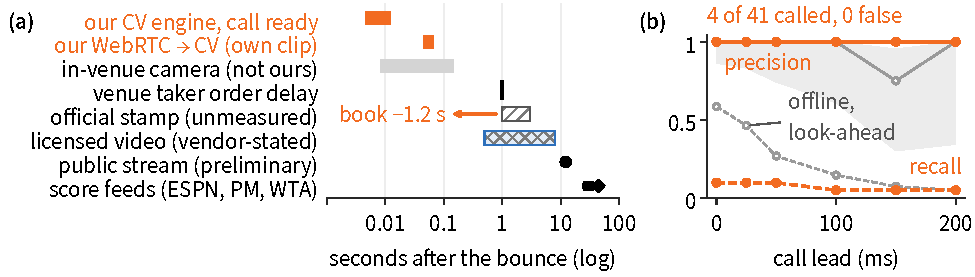
\includegraphics{../../results/paper/fig1_latency_cv.pdf}
\caption{\emph{The race is decided inside the venue's 1\,s taker delay; only in-venue information beats the book.}
(a)~Delay after the bounce (log): orange = ours (WebRTC: our own clip, loopback, 46 ms p50, 67 ms p99); hatched =
vendor-stated or model range. (b)~Early out-calls, held-out 120\,fps table-tennis video (41 out,
130 in; band: Wilson 95\%). Source: Polymarket and WTA feeds; \texttt{results/\{tracking,engine,webrtc\}}.}
\label{fig:ladder}
\end{figure}

\begin{figure}[t]
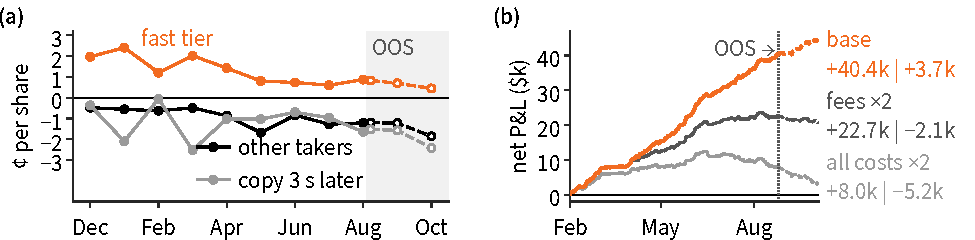
\includegraphics{../../results/paper/fig2_speed_edge.pdf}
\caption{\emph{Speed is the edge.} (a)~Monthly net 30\,s markout after fees; filled = IS, hollow = OOS. (b)~v2 net
P\&L at the fast tier's own fills (the opportunity at their speed, not our execution), base and costs doubled; solid =
IS, dashed = OOS; labels: IS\,|\,OOS totals. Source: \texttt{results/\{alpha,lowloss,v2\}}.}
\label{fig:edge}
\end{figure}

\begin{table}[b]
\caption{\emph{v2 earns in both periods at the fast tier's own fills; its OOS edge does not survive doubled fees.}}
\label{tab:v2}
\tabnums
\begin{tabular*}{\textwidth}{@{\extracolsep{\fill}}lrr@{}}
\toprule
 & In sample & Burned OOS \\
 & Feb 1--Aug 25, 206\,d & Aug 25--Oct 3, 40\,d \\
\midrule
Trades (matches) & 55,662 (7,639) & 10,412 (2,003) \\
Net ¢ per share [95\% CI] & +1.38 [1.17, 1.59] & +0.60 [0.09, 1.13] \\
Net edge\,/\,fee, bps of notional & 273\,/\,120 & 114\,/\,179 \\
Annualised return\,/\,volatility & 253\%\,/\,17.5\% & 148\%\,/\,22.2\% \\
Sharpe, annualised [bootstrap 95\% CI] & 14.5 [11.9, 17.4] & 6.7 [1.9, 12.3] \\
Max drawdown\,/\,worst day, \% of capital & −2.0\%\,/\,−1.9\% & −2.1\%\,/\,−2.1\% \\
Skew\,/\,worst month & +0.53\,/\,+\$2,543 & +0.33\,/\,−\$434 \\
Turnover (\(\times\) capital a year)\,/\,months positive & 93\,/\,7/7 & 129\,/\,2/3 \\
\textbf{Costs stressed:} ½\,/\,1 tick worse entry & +0.88\,/\,+0.38 & +0.10\,/\,−0.40 \\
\quad Fees \(\times\)2 [CI] (months positive) & +0.77 [0.57, 0.98] (7/7) & −0.34 [−0.86, 0.19] (0/3) \\
\quad All costs \(\times\)2 [CI] & +0.27 [0.07, 0.48] & −0.84 [−1.36, −0.31] \\
\bottomrule
\end{tabular*}
\tabnotes{\emph{Notes:} held to resolution, net of fees and spreads; capital 3\(\times\) peak locked
(\$28,302\,/\,\$22,754); CIs by match (by wallet, OOS: [−0.45, 2.38]).
\emph{Source:} \texttt{results/v2/}.}
\end{table}

% ======================================================================================== 5 Results
\section{Results}\label{sec:results}
The fast tier beats other takers every month and copying it 3\,s later loses (Fig.~\ref{fig:edge}a). At its fills v2
earns in both periods (Table~\ref{tab:v2}, Fig.~\ref{fig:edge}b); out of sample the edge is gone at ½ tick
worse entry (+0.10¢) and negative with fees doubled (−0.34¢,
0/3 months positive).
\para{Sharpe above 3} We assumed a bug and found one: fixing the onset look-ahead (D9) cut IS Sharpe from
16.8 to 14.5. The rest is about 270 small, nearly
independent bets a day (same-day correlation 0.0013). The deflated Sharpe \citep{bailey2014} is
0.997 IS at \(N = 3,386\) but 0.075–0.839 OOS: 40 days cannot rule out luck.
The CV Sharpe is a simulation's seed mean and ignores model risk.
\para{The 1\,s baseline} Table~\ref{tab:cv} and Fig.~\ref{fig:decay} give the main result. The two readings bracket it:
+\$57/day OOS (Sharpe 8.8) calibrated against +\$4/day
(Sharpe 0.3, −0.38¢ per share) pre-registered. Public streams and score feeds sit far
right of break-even; under the stamp-noise reading the trader loses at every \(V\) (Table~\ref{tab:A-usd}). A replay of 9 matches recorded live on 2026-10-03 against their real books
loses in 36 of 36 settings (−0.94¢ at \(V = 1\)\,s;
Fig.~\ref{fig:decay}d): it trades every point, not only \(\geq\)4¢ jumps; one day, an illustration.
Every blind test of a tradable book failed (Table~\ref{tab:fail}); the fast-minus-others gap stayed positive wherever measured.

\begin{figure}[t]
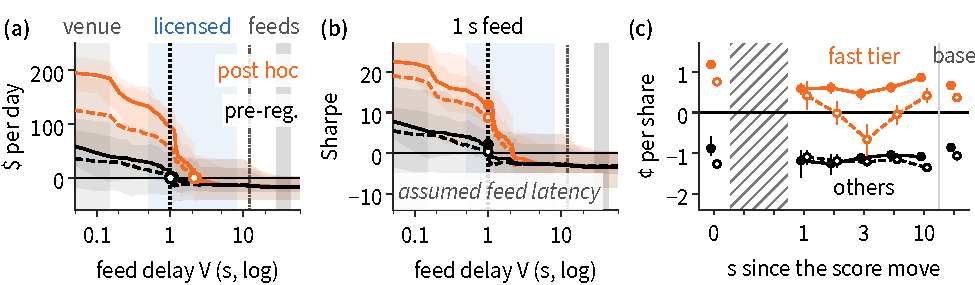
\includegraphics{../../results/paper/fig3_signal_decay.pdf}
\caption{\emph{Signal decay: each second of feed latency costs the edge.} (a)~\$/day, (b)~Sharpe against feed delay
\(V\) for both stamp lags; solid = IS, dashed = OOS; bands: 20 seeds; circles: break-even.
(c)~Net markout by seconds since the move. (d)~Replay of 9 live-recorded matches on real books;
\(\times\): sweep. Simulated at an assumed feed latency (licensed feed not purchased); parameters measured. Source: \texttt{results/\{tier0,decay,replay\}}.}
\label{fig:decay}
\end{figure}

\begin{table}[t]
\caption{\emph{Main result: simulated at a 1\,s licensed-feed baseline; assumed feed latency (licensed feed not purchased); parameters measured.}}
\label{tab:cv}
\tabnums
\begin{tabular*}{\textwidth}{@{\extracolsep{\fill}}lrrrr@{}}
\toprule
 & \multicolumn{2}{c}{Calibrated \(L = 3.14\)\,s (post hoc)} & \multicolumn{2}{c}{Pre-registered \(L = 2.0\)\,s} \\
\cmidrule(lr){2-3}\cmidrule(l){4-5}
At \(V = 1\)\,s & IS & OOS & IS & OOS \\
\midrule
Net \$ per day [seed 95\%] & +\$94 [51, 125] & +\$57 [1, 130] & +\$15 [−9, 43] & +\$4 [−36, 62] \\
Net ¢ per share & +1.11 & +0.66 & +0.40 & −0.38 \\
\quad 95\% CI & [0.85, 1.38] & [0.10, 1.19] & [−0.32, 1.08] & [−2.08, 1.21] \\
Sharpe, annualised & 11.9 & 8.8 & 2.1 & 0.3 \\
Ann. return\,/\,vol, \% & 118\,/\,9.9 & 91\,/\,10.3 & 30\,/\,14.1 & 11\,/\,33.4 \\
Max DD \%\,/\,worst day & −1.6\,/\,−\$223 & −1.6\,/\,−\$192 & −6.6\,/\,−\$263 & −5.3\,/\,−\$228 \\
Break-even \(V\), s [95\% CI] & 2.23 & 2.14 & 1.09 & 1.01 \\
 & [2.18, 3.39] & [1.59, 2.19] & [1.03, 2.04] & [0.43, 1.05] \\
\bottomrule
\end{tabular*}
\tabnotes{\emph{Notes:} means of 20 draws; IS: 1\,s-delay matches (103\,d); OOS burned
(40\,d); vol = return/Sharpe; 24--65 trades a day; no daily
path stored (equity curve: v2). At \(L = 1\)\,s: −\$6\,/\,−\$11 a day.}
\end{table}

\begin{table}[b]
\caption{\emph{Every blind test of a tradable book failed or is pending.}}
\label{tab:fail}
\tabnums
\begin{tabularx}{\textwidth}{@{}Xrrl@{}}
\toprule
Test, ¢ per share & IS & OOS or blind & Verdict \\
\midrule
H1\,\textperiodcentered\,H2\,\textperiodcentered\,H5 (post hoc) & −1.61\,\textperiodcentered\,−0.41\,\textperiodcentered\,+0.22 & −2.08\,\textperiodcentered\,+0.80\,\textperiodcentered\,+0.16 & fail\,\textperiodcentered\,none\,\textperiodcentered\,n.s. \\
v1 copy fast tier (OOS opened once) & +1.16 & +0.57 (−\$36,056) & fail \\
v2, 11,307 unseen markets (blind) & +2.02 & +1.22 [−0.19, 2.65] & fail \\
Tier-0 v3 rule, unseen markets (blind) & −0.22 & −0.52 & fail \\
Maker v1 (blind), per fill & +2.02 & +1.87 [−0.14, 3.86] & fail, −\$379 \\
v2 after fixed costs, \$ a day & +\$29 & −\$75 & fail OOS \\
Table tennis TT1--TT5, 27 matches & \multicolumn{2}{r}{no fast wallet qualifies} & untestable \\
Replay on live books, \(V = 1\)\,s & & −0.94 [−1.28, −0.58] & loses \\
Forward test\,\textperiodcentered\,live paper session & & \multicolumn{2}{r}{pending\,\textperiodcentered\,pending} \\
\bottomrule
\end{tabularx}
\tabnotes{\emph{Notes:} \textbf{4,219 variants tried} (Table~\ref{tab:A-var}). Fast minus others,
unseen markets: +3.09\,/\,+2.16¢ (the latency gap held). Held-out data read 69 times
(7 blind first runs, 13 non-blind, 5 descriptive,
22 audits, 20 replay/live, 2 other; Table~\ref{tab:A-peeks});
rules changed after a look 2 times.}
\end{table}

% ======================================================================================== 6 Risk
\section{Risk management}\label{sec:risk}
\begin{itemize}
\item \textbf{Limits.} \$1,000 per order, 100 shares net per match, zone
0.05–0.95; capital 3\(\times\) peak locked (\$28,302); worst day −\$551\,/\,−\$469
(IS\,/\,OOS). Kill switches in code (\texttt{engine/risk/}): daily stop \$1,000
(3.86\,\(\sigma\)), stale feed \(>\)2\,s or vision
\(>\)1\,s, latency above its rolling p95.
\item \textbf{De-risking, set in advance.} Halve size if the trailing 30-day edge is below 0.3¢
(IS minimum +0.74¢); stop at \(\leq 0\), at a 5\% drawdown, or on a fee or delay change.
\item \textbf{Largest risks.} Venue rules (doubled fees erase the OOS edge); crowding (top five wallets:
81\%\,/\,142\% of P\&L); tails (kurtosis 4.30\,/\,3.26);
legal (courtsiding breaches ticket terms, \citealp{itf2026}). Factors \citep{fama1993,carhart1997}: \(\alpha\)
\(t = 8.48\), max \(|t| = 1.36\), R² 3.3\% (IS; Table~\ref{tab:A-factor}).
\end{itemize}

% ======================================================================================== 7 Liquidity
\section{Liquidity and capacity}\label{sec:liq}
v2 trades \$7,182 a day, 0.07\% of match volume. Its OOS per-share CI
excludes zero only up to 1\(\times\) size (\$22,754 of capital); 2\(\times\) spans zero and
5\(\times\) loses (Fig.~\ref{fig:cap}a). Median stale depth before a reprice: \$222,
\$379, \$564 at 0, 1, 2\,s; spread 1¢. Fees bind: the OOS
break-even fee is 8.2\%, or 2.4\% after an assumed
\$5,000-a-month feed licence, which takes the 1\,s-baseline OOS P\&L to
−\$110 (calibrated) or −\$163 (pre-registered) a day (Fig.~\ref{fig:cap}b).

% ======================================================================================== 8 Limitations
\section{Limitations and next steps}\label{sec:limits}
The key uncertainty is the stamp lag \(L\) (Eq.~\ref{eq:budget}), which moves the break-even one for one; one live
session with a licensed low-latency feed, timing bounce against stamp, would measure it. Licensing that feed turns the
simulation into deployment (Polymarket US already licenses official data and live streams: Genius Sports for selected
leagues, ATP Tour streaming rights; \citealp{gi2026,prn2026}); a faster feed moves left on the curve
(Fig.~\ref{fig:decay}a); then an organiser-consented venue camera. Risks: fee rises, a longer delay, faster rivals,
wallet exits, legal access. Table tennis is illiquid (median spread 94¢).\label{lastmain}

% ======================================================================================== References
\clearpage
\renewcommand\refname{References}
\bibliographystyle{apalike}
{\setlength\bibsep{2pt}\bibliography{refs}}
\nocite{harvey2016,politis1994,bailey2017,harvey2017,huang2019,statsperform,nextio,sportradar,ably,regen2026,glsystemhaus,ispreview,thedesk,itia2026}

\vspace{6pt}\noindent\textbf{Disclosure.} No real money was used. Simulated components are labelled. The authors hold no
licensed data feed, no match footage and no court access. University of Florida students; [team to confirm any other
disclosures].

% ======================================================================================== Appendix
\clearpage
\csappendix
\section*{Appendix}
\addcontentsline{toc}{section}{Appendix}
Everything a judge needs for scoring is in the five main pages; this appendix gives the full grids, logs and tallies
behind them. Every appendix float repeats its label.

\begin{figure}[!ht]
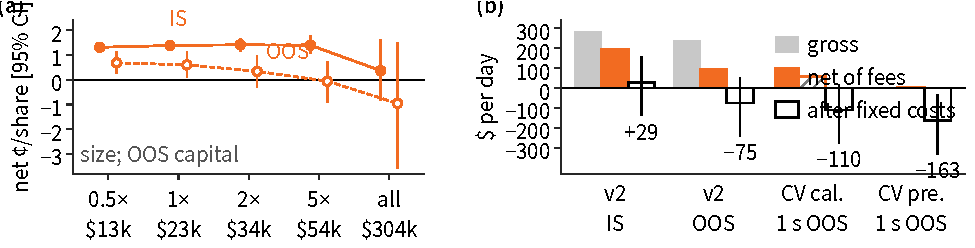
\includegraphics{../../results/paper/figA1_capacity.pdf}
\caption{\emph{Capacity is small and costs bind.} (a)~v2 net edge by size (caps scaled; optimistic at large size); filled
= IS, hollow = OOS. (b)~\$/day: gross, net of fees, after fixed costs (low--high); CV: 1\,s baseline, OOS,
assumed feed latency (licensed feed not purchased); parameters measured. Source: \texttt{results/financials}.}
\label{fig:cap}
\end{figure}

\begin{table}[!ht]
\caption{\emph{Latency sweep, every reading: Net \$ per day against feed delay \(V\) (s), IS and burned OOS.} Simulated:
assumed feed latency (licensed feed not purchased); parameters measured.}
\label{tab:A-usd}
\tabnums
\setlength\tabcolsep{4pt}
\begin{tabular*}{\textwidth}{@{\extracolsep{\fill}}llrrrrrrr@{}}
\toprule
Stamp lag reading & & 0 & 0.5 & 1 & 2 & 5 & 10 & 60 \\
\midrule
calibrated 3.14 s (post hoc) & IS & 199 & 133 & 94 & 15 & −13 & −13 & −17 \\
 & OOS & 129 & 81 & 57 & 7 & −13 & −13 & −17 \\
pre-registered 2.0 s & IS & 89 & 28 & 15 & −6 & −13 & −14 & −17 \\
 & OOS & 46 & 15 & 4 & −11 & −13 & −13 & −17 \\
stress 1.0 s & IS & 15 & −5 & −6 & −13 & −13 & −14 & −17 \\
 & OOS & 4 & −11 & −11 & −13 & −13 & −13 & −17 \\
lag 3.0 s & IS & 189 & 121 & 89 & 15 & −13 & −13 & −17 \\
 & OOS & 117 & 76 & 46 & 4 & −13 & −13 & −17 \\
stamp-noise reading & IS & −30 & −17 & −17 & −17 & −17 & −17 & −17 \\
 & OOS & −26 & −17 & −17 & −17 & −17 & −17 & −17 \\
stamp-noise, calibrated & IS & 199 & −45 & −17 & −17 & −17 & −17 & −17 \\
 & OOS & 133 & −40 & −17 & −17 & −17 & −17 & −17 \\
\bottomrule
\end{tabular*}
\tabnotes{\emph{Notes:} seed means over 20 draws per cell (18,880 runs in all). The
stamp-noise readings spread the reprice time by umpire-stamp noise instead of by tournament. \emph{Source:}
\texttt{results/tier0/latency\_sweep.json::video\_own120}.}
\end{table}
\begin{table}[!ht]
\caption{\emph{Latency sweep, every reading: Annualised Sharpe against feed delay \(V\) (s), IS and burned OOS.} Simulated:
assumed feed latency (licensed feed not purchased); parameters measured.}
\label{tab:A-sr}
\tabnums
\setlength\tabcolsep{4pt}
\begin{tabular*}{\textwidth}{@{\extracolsep{\fill}}llrrrrrrr@{}}
\toprule
Stamp lag reading & & 0 & 0.5 & 1 & 2 & 5 & 10 & 60 \\
\midrule
calibrated 3.14 s (post hoc) & IS & 22.9 & 15.5 & 11.9 & 2.2 & −2.7 & −2.7 & −3.4 \\
 & OOS & 19.6 & 12.2 & 8.8 & 0.9 & −2.6 & −2.6 & −3.2 \\
pre-registered 2.0 s & IS & 11.4 & 4.0 & 2.1 & −1.4 & −2.7 & −2.9 & −3.4 \\
 & OOS & 7.3 & 2.1 & 0.3 & −2.3 & −2.6 & −2.6 & −3.2 \\
stress 1.0 s & IS & 2.1 & −1.3 & −1.4 & −2.6 & −2.7 & −2.9 & −3.4 \\
 & OOS & 0.3 & −2.3 & −2.3 & −2.6 & −2.6 & −2.6 & −3.2 \\
lag 3.0 s & IS & 21.8 & 14.4 & 11.4 & 2.1 & −2.7 & −2.7 & −3.4 \\
 & OOS & 17.5 & 11.4 & 7.3 & 0.3 & −2.6 & −2.6 & −3.2 \\
stamp-noise reading & IS & −5.9 & −3.4 & −3.4 & −3.4 & −3.4 & −3.4 & −3.4 \\
 & OOS & −5.0 & −3.2 & −3.2 & −3.2 & −3.2 & −3.2 & −3.2 \\
stamp-noise, calibrated & IS & 25.1 & −8.7 & −3.4 & −3.4 & −3.4 & −3.4 & −3.4 \\
 & OOS & 21.2 & −7.6 & −3.2 & −3.2 & −3.2 & −3.2 & −3.2 \\
\bottomrule
\end{tabular*}
\tabnotes{\emph{Notes:} seed means over 20 draws per cell (18,880 runs in all). The
stamp-noise readings spread the reprice time by umpire-stamp noise instead of by tournament. \emph{Source:}
\texttt{results/tier0/latency\_sweep.json::video\_own120}.}
\end{table}

\begin{figure}[!ht]
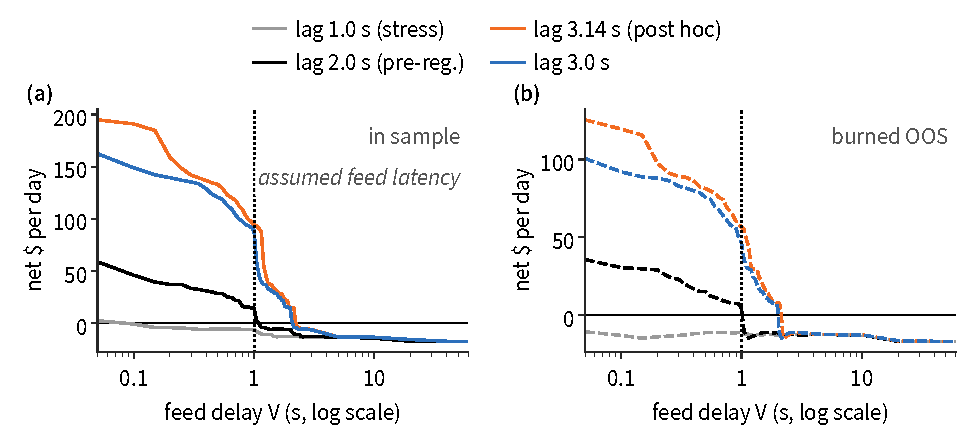
\includegraphics{../../results/paper/figA2_sweep_lags.pdf}
\caption{\emph{The break-even shifts one for one with the stamp lag.} Net \$/day against feed delay for every stamp-lag
reading, (a)~IS and (b)~burned OOS. Simulated: assumed feed latency (licensed feed not purchased); parameters measured. Source: \texttt{results/tier0/latency\_sweep.csv}.}
\end{figure}

\begin{figure}[!ht]
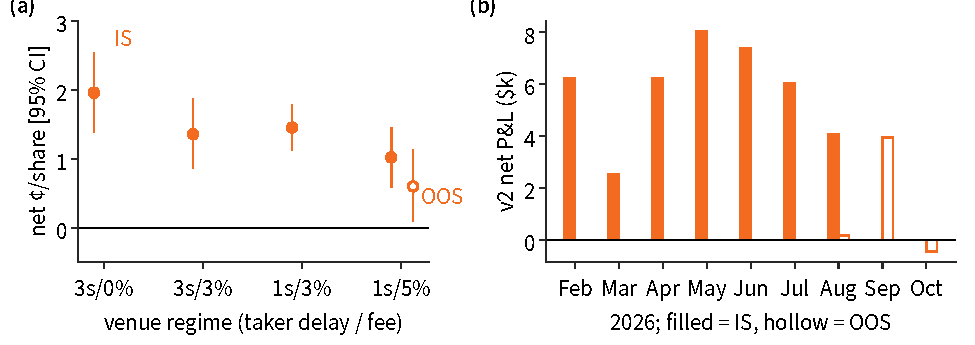
\includegraphics{../../results/paper/figA3_regime_month.pdf}
\caption{\emph{v2's edge falls as the venue's protection falls, and stays positive in every in-sample regime.}
(a)~Net ¢ per share by venue regime (taker delay\,/\,fee) with 95\% CIs; (b)~net P\&L by month. Measured at the fast
tier's own fills: the opportunity at their speed, not our execution. Source: \texttt{results/risk/risk\_stats.json}.}
\end{figure}

\begin{figure}[!ht]
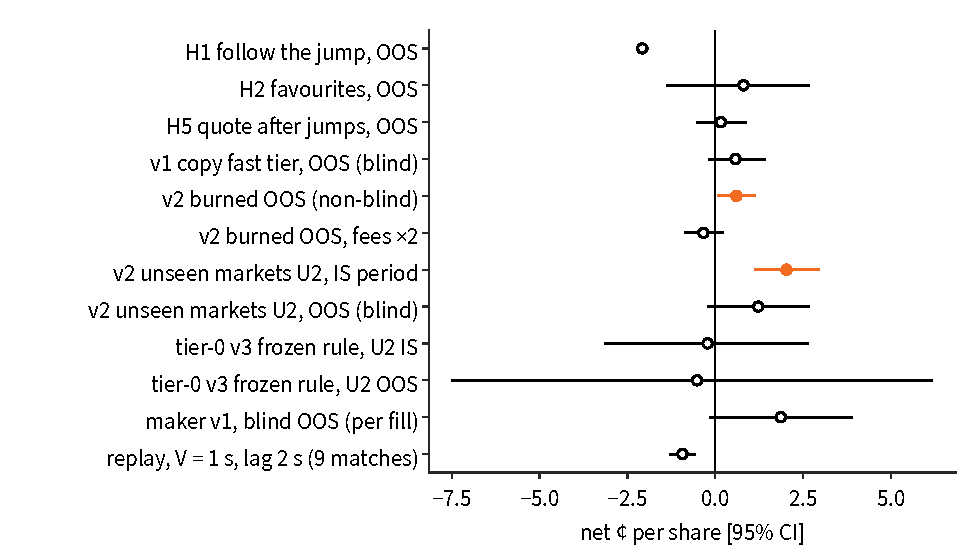
\includegraphics{../../results/paper/figA4_forest.pdf}
\caption{\emph{Every test on one axis.} Point estimates and 95\% CIs, net ¢ per share; orange = CI above zero, hollow = the test failed or has no edge. Source: as Table~\ref{tab:fail}.}
\end{figure}

\begin{figure}[!ht]
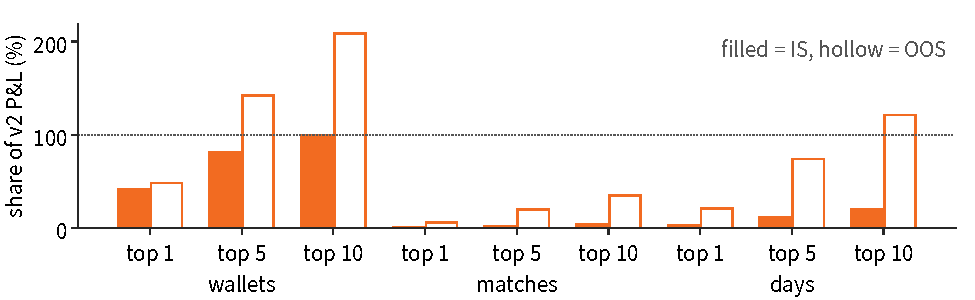
\includegraphics{../../results/paper/figA5_concentration.pdf}
\caption{\emph{v2 P\&L is concentrated in a few copied wallets.} Share of v2 P\&L carried by the top 1, 5 and 10
wallets, matches and days (above 100\% means the rest lost money). Source: \texttt{results/alpha/alpha.json}.}
\end{figure}

\begin{figure}[!ht]
\centering
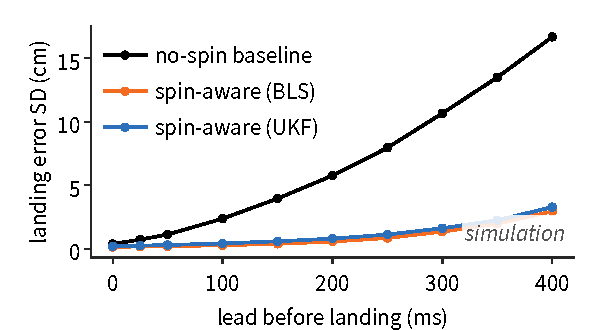
\includegraphics{../../results/paper/figA6_spin_sim.pdf}
\caption{\emph{Simulation: a spin-aware tennis filter cuts landing error.} Landing-point error against lead before the
bounce for a 340\,fps, 3.6\,mm-noise ball tracker (simulation; no tennis video was used). At 200\,ms:
5.76\,cm without spin, 0.57\,cm with it. Source:
\texttt{results/spin/tennis/key\_numbers.json}.}
\end{figure}

\clearpage
\begin{table}[!ht]
\caption{\emph{Factor regressions: v2's daily return has no meaningful equity-factor exposure.} Fama--French three
factors plus momentum, Newey--West 5 lags.}
\label{tab:A-factor}
\tabnums\setlength\tabcolsep{3pt}
\begin{tabular*}{\textwidth}{@{\extracolsep{\fill}}lrrrrrrr@{}}
\toprule
Specification & \(\alpha\) \%/day (\(t\)) & Mkt (\(t\)) & SMB (\(t\)) & HML (\(t\)) & Mom (\(t\)) & \(R^2\) & days \\
\midrule
IS only (headline) & 0.80 (8.5) & 0.17 (1.4) & 0.08 (0.5) & 0.04 (0.4) & 0.03 (0.4) & 3.3\% & 138 \\
IS, calendar days & 0.68 (9.5) & -- & -- & -- & -- & 2.3\% & 206 \\
File (5 OOS days) & 0.79 (8.5) & 0.17 (1.3) & 0.09 (0.5) & 0.06 (0.6) & 0.03 (0.5) & 3.3\% & 142 \\
\bottomrule
\end{tabular*}
\tabnotes{\emph{Notes:} the committed file includes five burned-OOS weekdays and is shown only for completeness.
\emph{Source:} \texttt{results/alpha/alpha.json::C\_factor\_neutral}; \citet{french}.}
\end{table}

\begin{table}[!ht]
\caption{\emph{Variant tally: 4,219 configurations tried; the sensitivities chose nothing.}}
\label{tab:A-var}
\begin{tabularx}{\textwidth}{@{}Xrl@{}}
\toprule
Family & Count & What it chose \\
\midrule
H1-H6 pre-registered and H5/H6 rules & 44 & frozen primaries (DEVIATIONS D6) \\
v2 lenses (exit, sizing, selection, cross-market, latency, Kalshi) & 3,342 & v2 (G\_50pct\_net100), IS only \\
v2-safe grid & 24 & v2-safe (secondary) \\
tier-0 pre-registered scenarios & 432 & none (sensitivity grid) \\
tier-0 v3 in-sample grid & 360 & frozen v3 rule (blind: FAIL) \\
maker v1 evaluated variants & 8 & maker v1 primary (blind: FAIL) \\
cost-stress cases & 4 & none (stress) \\
table-tennis tests TT1-TT5 & 5 & none (untestable) \\
\midrule
\textbf{Total} & \textbf{4,219} & \\
\emph{Sensitivity, chose nothing:} latency-sweep cells & 944 & none \\
\emph{Sensitivity, chose nothing:} replay cells & 36 & none \\
\bottomrule
\end{tabularx}
\tabnotes{\emph{Source:} \texttt{results/paper/variants.json} (each count's source file is listed there).}
\end{table}

\begin{table}[!ht]
\caption{\emph{Fixed-cost assumptions behind Fig.~\ref{fig:cap}b (\$ per month unless stated).}}
\label{tab:A-costs}
\tabnums
\begin{tabularx}{\textwidth}{@{}Xrrrl@{}}
\toprule
Item & Low & Central & High & Label \\
\midrule
Official live ATP/WTA point-data feed licence & \$1,250 & \$5,000 & \$10,000 & ASSUMPTION \\
London gateway VPS (AWS eu-west-2, on-demand Linux) & \$34 & \$77 & \$98 & ESTIMATE \\
Polymarket CLOB / data API & \$0 & \$0 & \$0 & ESTIMATE \\
HiPerGator (training, backtests) & \$0 & \$0 & \$0 & ESTIMATE \\
Courtside camera operator (tier-0 only) & \$36 & \$36 & \$36 & ESTIMATE \\
Cloud GPU for CV inference, per covered event hour (tier-0 only) & \$1 & \$1 & \$1 & ESTIMATE \\
Operator + GPU hours per covered match (tier-0 only) & \$3 & \$4 & \$5 & ASSUMPTION \\
Camera position / venue access fee per event (tier-0 only) & \$0 & \$250 & \$500 & ASSUMPTION \\
120 fps camera kit, amortised over 24 months (tier-0 only) & \$648 & \$1,000 & \$2,000 & ESTIMATE \\
\bottomrule
\end{tabularx}
\tabnotes{\emph{Notes:} no public price exists for an official low-latency tennis feed; the range is anchored to
reported figures (bases and URLs in the source file). \emph{Source:}
\texttt{results/financials/financials.json::cost\_assumptions}.}
\end{table}

\begin{table}[!ht]
\caption{\emph{The latency ladder: method and source of every row of Fig.~\ref{fig:ladder}a.}}
\label{tab:A-ladder}
\begin{tabularx}{\textwidth}{@{}lrX@{}}
\toprule
Source & Delay & Method and citation \\
\midrule
Our CV engine, call-ready (p50--p99) & 4.6--12.2\,ms & measured, one L4 GPU, 120\,fps held-out video \\
Our WebRTC \(\to\) CV pipeline & 46 ms p50, 67 ms p99 & measured: our own clip over loopback, frame send to call (55 calls; engine fed below real time so it keeps up); not a match feed \\
Network, Florida \(\to\) venue gateway & 67\,ms & measured (live feed p50 65\,ms) \\
In-venue camera & \(\leq\)0.15\,s & physical bound; not available to us \\
Venue taker order delay & 1\,s & venue rule \citep{pmapi} \\
Official umpire stamp after the bounce & 1–3\,s & unmeasured model grid \citep{regen2026,statsperform} \\
Book reprice vs official stamp & \(-\)1.2\,s & measured median, \(n = 482\) \\
Licensed betting video & 0.5–8\,s & vendor claims, unverified, none for tennis \citep{statsperform,nextio,sportradar,ably} \\
Fastest public stream of a listed match & 12.2\,s & measured, preliminary (no YouTube-derived figure used) \\
ESPN\,/\,PM sports\,/\,WTA vs book & 28.2\,/\,30.0\,/\,44.1\,s & measured medians, 2026-10-03 \citep{espn,wtaapi} \\
TV and public streams, general & 0.9--60\,s & published comparisons \citep{ispreview,glsystemhaus,thedesk} \\
\bottomrule
\end{tabularx}
\tabnotes{\emph{Source:} \texttt{research/v2/latency/results.json}, \texttt{results/tier0/latency\_sweep.json::sources},
\texttt{results/home\_stream/sub\_second\_routes.json}, \texttt{results/engine/online\_vs\_offline.json}.}
\end{table}

\clearpage
\begin{longtable}{@{}p{0.85in}p{0.95in}p{4.35in}@{}}
\caption{\emph{Every logged read of held-out data (69 lines of \texttt{results/oos\_peeks.log} at build
time), with its class.}}\label{tab:A-peeks}\\
\toprule
UTC & Class & What was read (truncated) \\
\midrule
\endfirsthead
\toprule
UTC & Class & What was read (truncated) \\
\midrule
\endhead
\bottomrule
\endfoot
10-03 10:42 & other & OOS prints built \\
10-03 13:24 & non-blind & v2 evaluated on burned OOS (non-\allowbreak{}blind,\allowbreak{} labelled) \\
10-03 13:53 & non-blind & v2-\allowbreak{}causal (D9 fix) evaluated on burned OOS (non-\allowbreak{}blind) \\
10-03 17:23 & non-blind & tier0 counterfactual: OOS jump table built (burned OOS,\allowbreak{} non-\allowbreak{}blind) \\
10-03 17:29 & non-blind & tier0 counterfactual grid evaluated on burned OOS (non-\allowbreak{}blind,\allowbreak{} labelled) \\
10-03 17:31 & blind first run & U2 out-\allowbreak{}of-\allowbreak{}universe test evaluated (PREREG research/\allowbreak{}v2/\allowbreak{}expand,\allowbreak{} first run) \\
10-03 17:37 & non-blind & v2-\allowbreak{}safe (lowloss PREREG) evaluated on burned OOS (non-\allowbreak{}blind,\allowbreak{} labelled) \\
10-03 17:37 & blind first run & v2-\allowbreak{}safe U2 out-\allowbreak{}of-\allowbreak{}universe test evaluated (PREREG research/\allowbreak{}v2/\allowbreak{}lowloss,\allowbreak{} first run) \\
10-03 17:43 & audit & tier0 independent rebuild: OOS prints read for jump onsets + stale price (burned OOS,\allowbreak{} non-\allowbreak{}blind,\allowbreak{} labelled) \\
10-03 17:45 & audit & tier0 independent rebuild: OOS prints read for jump onsets + stale price (burned OOS,\allowbreak{} non-\allowbreak{}blind,\allowbreak{} labelled) \\
10-03 17:48 & audit & tier0 independent rebuild: OOS prints read for jump onsets + stale price (burned OOS,\allowbreak{} non-\allowbreak{}blind,\allowbreak{} labelled) \\
10-03 18:00 & non-blind & v2 cost stress (fees/\allowbreak{}costs doubled,\allowbreak{} book fixed) on burned OOS (non-\allowbreak{}blind,\allowbreak{} no parameter change) \\
10-03 18:06 & non-blind & tier0 corrections: OOS post-\allowbreak{}jump prices built (burned OOS,\allowbreak{} non-\allowbreak{}blind,\allowbreak{} labelled) \\
10-03 18:13 & non-blind & tier0 counterfactual (verifier corrections) evaluated on burned OOS (non-\allowbreak{}blind,\allowbreak{} labelled) \\
10-03 18:27 & descriptive & maker venue rules: descriptive in-\allowbreak{}play book spread/\allowbreak{}depth + tick changes read from data/\allowbreak{}live\_\allowbreak{}v2 forward recordings (no strategy,\allowbreak{} no P\&L,\allowbreak{} no parameter c\ldots \\
10-03 18:42 & non-blind & financials: v2 /\allowbreak{} v2-\allowbreak{}safe size-\allowbreak{}scaled variants (0.5x,\allowbreak{} 2x,\allowbreak{} 5x,\allowbreak{} all prints) evaluated on burned OOS (non-\allowbreak{}blind,\allowbreak{} capacity curve only) \\
10-03 18:47 & descriptive & maker live engine plumbing: data/\allowbreak{}live\_\allowbreak{}v2 clob\_\allowbreak{}17/\allowbreak{}clob\_\allowbreak{}13 read for message ordering only (price\_\allowbreak{}change vs last\_\allowbreak{}trade\_\allowbreak{}price timestamps,\allowbreak{} trade dedupe); n\ldots \\
10-03 18:49 & blind first run & maker v1 blind OOS evaluated (first run) (PREREG research/\allowbreak{}v2/\allowbreak{}maker/\allowbreak{}PREREG.md (A); first use of OOS side-\allowbreak{}market tapes; burned OOS moneyline tapes used \ldots \\
10-03 18:49 & audit & maker v1 OOS reproduction (recompute committed results.json; no parameter change) \\
10-03 19:00 & live & maker v1 live paper engine REPLAY (recorded live data) on data/\allowbreak{}live\_\allowbreak{}v2/\allowbreak{}clob\_\allowbreak{}20261003\_\allowbreak{}1123\_\allowbreak{}20261003\_\allowbreak{}11.jsonl.gz,\allowbreak{}data/\allowbreak{}live\_\allowbreak{}v2/\allowbreak{}clob\_\allowbreak{}20261003\_\allowbreak{}1123\_\allowbreak{}2026100\ldots \\
10-03 19:13 & live & maker v1 live paper TEST run (not the pre-\allowbreak{}registered session) START: run=20261003T190317Z commit=56a9c8f77b1aaf7b1306c2f1b06d6a2e05c798a8+dirty until=\ldots \\
10-03 19:15 & audit & P17 clean-\allowbreak{}clone reproduce.sh (HEAD 56a9c8f,\allowbreak{} scratch clone,\allowbreak{} data/\allowbreak{} linked,\allowbreak{} backtest workers=1): re-\allowbreak{}runs the committed frozen scripts incl. run\_\allowbreak{}all.py -\allowbreak{}-\allowbreak{}\ldots \\
10-03 19:19 & live & maker v1 live paper engine REPLAY (B2: own raw log) on data/\allowbreak{}live\_\allowbreak{}maker/\allowbreak{}raw\_\allowbreak{}20261003T190317Z.jsonl.gz window=-\allowbreak{}+Nonemin clock=recv: run=20261003T191913Z\ldots \\
10-03 19:20 & non-blind & PM review P07: wallet-\allowbreak{}clustered bootstrap CI of the frozen v2 causal book on burned OOS (non-\allowbreak{}blind,\allowbreak{} labelled; the CI the note already quotes,\allowbreak{} no rule \ldots \\
10-03 19:23 & blind first run & table tennis TT1-\allowbreak{}TT4 evaluated (first run) \\
10-03 19:25 & descriptive & TT5 signal decay (scripts/\allowbreak{}signal\_\allowbreak{}decay.py,\allowbreak{} commit a5769c786f935dcc05ff2ab90a1947ad0cde4cb5+dirty(signal\_\allowbreak{}decay.py)): reads table tennis UTT OOS prints \ldots \\
10-03 19:28 & other & table tennis post-\allowbreak{}hoc diagnostics after TT1-\allowbreak{}TT4 (closing-\allowbreak{}print size,\allowbreak{} fast-\allowbreak{}tier distance; not pre-\allowbreak{}registered,\allowbreak{} no verdict change) \\
10-03 19:28 & live & maker v1 live paper TEST run (not the pre-\allowbreak{}registered session) START: run=20261003T191915Z commit=ad164da6da24325afcfdbab8fe24dcf5f0516fed+dirty until=\ldots \\
10-03 19:58 & live & maker v1 live paper session (B) START: run=20261003T193534Z commit=114c722e6b203421d8b4f55a5da2b54a1658b658 until=2026-\allowbreak{}10-\allowbreak{}04T11:30:00.000Z (PREREG res\ldots \\
10-03 20:02 & audit & audit: independent TT3 reproduction (research/\allowbreak{}tt/\allowbreak{}audit\_\allowbreak{}tt3.py; reads UTT IS+OOS tapes/\allowbreak{}prints,\allowbreak{} already evaluated in 2195e86) plus labelled post-\allowbreak{}hoc dia\ldots \\
10-03 20:03 & audit & audit: table tennis checks (research/\allowbreak{}tt/\allowbreak{}audit\_\allowbreak{}checks.py): provenance,\allowbreak{} fees/\allowbreak{}delays,\allowbreak{} voids,\allowbreak{} counts,\allowbreak{} liquidity; reproduces TT1 closing bins (IS+OOS,\allowbreak{} alre\ldots \\
10-03 20:04 & audit & audit: financials/\allowbreak{}risk audit (scripts/\allowbreak{}financials\_\allowbreak{}audit.py) re-\allowbreak{}reads the frozen v2 burned-\allowbreak{}OOS trades and maker blind-\allowbreak{}OOS fills to reproduce numbers alr\ldots \\
10-03 20:07 & audit & audit: RE-\allowbreak{}RUN of research/\allowbreak{}tt/\allowbreak{}audit\_\allowbreak{}tt3.py with three added post-\allowbreak{}hoc counts (closest wallet's share of TT2 others' prints,\allowbreak{} 0-\allowbreak{}3 s prints at fav >= 0.95 \ldots \\
10-03 20:07 & audit & audit: RE-\allowbreak{}RUN of research/\allowbreak{}tt/\allowbreak{}audit\_\allowbreak{}tt3.py (traceback location recorded as repo-\allowbreak{}relative src/\allowbreak{}v2.py frames only; same reads and numbers,\allowbreak{} no rule or verd\ldots \\
10-03 20:09 & descriptive & alpha breakdown: descriptive splits of existing v2 trades incl. burned OOS (no parameter change) \\
10-03 20:10 & live & maker v1 live paper engine REPLAY (recorded live data) on data/\allowbreak{}live\_\allowbreak{}v2/\allowbreak{}clob\_\allowbreak{}20261003\_\allowbreak{}1123\_\allowbreak{}20261003\_\allowbreak{}1[12].jsonl.gz window=2026-\allowbreak{}10-\allowbreak{}03T12:00:00.000Z+60.0\ldots \\
10-03 20:10 & live & maker v1 live paper engine REPLAY (recorded live data) on data/\allowbreak{}live\_\allowbreak{}v2/\allowbreak{}clob\_\allowbreak{}20261003\_\allowbreak{}1123\_\allowbreak{}20261003\_\allowbreak{}1[12].jsonl.gz window=2026-\allowbreak{}10-\allowbreak{}03T12:00:00.000Z+60.0\ldots \\
10-03 20:11 & audit & audit: maker v1 blind OOS (A) independent recompute (own code in scratchpad,\allowbreak{} no import of scripts/\allowbreak{}maker\_\allowbreak{}oos.py or research/\allowbreak{}v2/\allowbreak{}maker/\allowbreak{}oos\_\allowbreak{}*.py); reads O\ldots \\
10-03 20:13 & live & maker v1 live paper engine REPLAY (recorded live data) on data/\allowbreak{}live\_\allowbreak{}v2/\allowbreak{}clob\_\allowbreak{}20261003\_\allowbreak{}1123\_\allowbreak{}20261003\_\allowbreak{}1[123].jsonl.gz window=2026-\allowbreak{}10-\allowbreak{}03T13:00:00.000Z+60.\ldots \\
10-03 20:13 & live & maker v1 live paper engine REPLAY (recorded live data) on data/\allowbreak{}live\_\allowbreak{}v2/\allowbreak{}clob\_\allowbreak{}20261003\_\allowbreak{}1123\_\allowbreak{}20261003\_\allowbreak{}1[1234].jsonl.gz window=2026-\allowbreak{}10-\allowbreak{}03T14:00:00.000Z+12\ldots \\
10-03 20:14 & live & maker v1 live paper engine REPLAY (recorded live data) on data/\allowbreak{}live\_\allowbreak{}v2/\allowbreak{}clob\_\allowbreak{}20261003\_\allowbreak{}1123\_\allowbreak{}20261003\_\allowbreak{}11.jsonl.gz window=2026-\allowbreak{}10-\allowbreak{}03T11:35:00.000Z+25.0min\ldots \\
10-03 20:14 & live & maker v1 live paper engine REPLAY (recorded live data) on data/\allowbreak{}live\_\allowbreak{}v2/\allowbreak{}clob\_\allowbreak{}20261003\_\allowbreak{}1123\_\allowbreak{}20261003\_\allowbreak{}1[56789].jsonl.gz window=2026-\allowbreak{}10-\allowbreak{}03T16:00:00.000Z+2\ldots \\
10-03 20:16 & non-blind & tier0 latency sweep on burned OOS (non-\allowbreak{}blind,\allowbreak{} labelled; no parameter chosen) \\
10-03 20:16 & audit & audit: TT5 same-\allowbreak{}block split and v2 trade join (research/\allowbreak{}decay/\allowbreak{}audit\_\allowbreak{}sameblock.py): re-\allowbreak{}reads tennis U1 IS + burned OOS prints (non-\allowbreak{}blind,\allowbreak{} already evalu\ldots \\
10-03 20:18 & audit & audit: selection check for maker v1 OOS (A): data-\allowbreak{}api /\allowbreak{}trades counts and notional (no prices used,\allowbreak{} no signal,\allowbreak{} no P\&L) for a random sample of 60 OOS si\ldots \\
10-03 20:21 & audit & audit: maker v1 OOS (A) stress (viii) alternative fee reading (makerBaseFee 1000 bps x min(px,\allowbreak{}1-\allowbreak{}px),\allowbreak{} CTF-\allowbreak{}exchange form) on the already-\allowbreak{}evaluated book-\allowbreak{}\ldots \\
10-03 20:22 & audit & audit: provenance spot-\allowbreak{}check of maker v1 OOS cache: re-\allowbreak{}download 8 cached OOS side tapes (data-\allowbreak{}api) and 1 Gamma events batch and compare with the cache\ldots \\
10-03 20:22 & live & maker v1 live paper engine REPLAY (B2: own raw log) on data/\allowbreak{}live\_\allowbreak{}maker/\allowbreak{}raw\_\allowbreak{}20261003T191915Z.jsonl.gz window=-\allowbreak{}+Nonemin clock=recv: run=20261003T202228Z\ldots \\
10-03 20:22 & live & maker v1 live paper engine REPLAY (B2: own raw log) on /\allowbreak{}private/\allowbreak{}tmp/\allowbreak{}claude-\allowbreak{}501/\allowbreak{}-\allowbreak{}Users-\allowbreak{}ojasvamishra32-\allowbreak{}Library-\allowbreak{}Application-\allowbreak{}Support-\allowbreak{}Claude-\allowbreak{}scratch-\allowbreak{}worksp\ldots \\
10-03 20:24 & non-blind & tier0 latency sweep on burned OOS (non-\allowbreak{}blind,\allowbreak{} labelled; no parameter chosen) \\
10-03 20:25 & audit & tier0 v3 blind test (a) burned OOS START (scripts/\allowbreak{}tier0\_\allowbreak{}v3\_\allowbreak{}blind.py; PREREG research/\allowbreak{}v2/\allowbreak{}tier0\_\allowbreak{}v3/\allowbreak{}PREREG.md section 5; non-\allowbreak{}blind window seen by v1/\allowbreak{}v2/\allowbreak{}t\ldots \\
10-03 20:26 & blind first run & tier0 v3 blind test (b) U2 START (scripts/\allowbreak{}tier0\_\allowbreak{}v3\_\allowbreak{}blind.py; PREREG research/\allowbreak{}v2/\allowbreak{}tier0\_\allowbreak{}v3/\allowbreak{}PREREG.md section 4; first tier-\allowbreak{}0 table on U2: jump tables + \ldots \\
10-03 20:28 & blind first run & tier0 v3 blind tests (a)+(b) DONE: burned OOS FAIL,\allowbreak{} U2-\allowbreak{}IS FAIL,\allowbreak{} U2-\allowbreak{}OOS FAIL -\allowbreak{}> results/\allowbreak{}tier0\_\allowbreak{}v3/\allowbreak{}blind.json \\
10-03 20:29 & blind first run & tier0 v3 blind tests (a)+(b) DONE: burned OOS FAIL,\allowbreak{} U2-\allowbreak{}IS FAIL,\allowbreak{} U2-\allowbreak{}OOS FAIL -\allowbreak{}> results/\allowbreak{}tier0\_\allowbreak{}v3/\allowbreak{}blind.json \\
10-03 20:37 & audit & audit: tier-\allowbreak{}0 v3 blind tests adversarial audit (independent code in scratchpad; COUNTERFACTUAL): re-\allowbreak{}reads saved v3 burned-\allowbreak{}OOS/\allowbreak{}U2 outputs (results/\allowbreak{}tier\ldots \\
10-03 20:40 & live & maker v1 live paper engine REPLAY (recorded live data) on data/\allowbreak{}live\_\allowbreak{}v2/\allowbreak{}clob\_\allowbreak{}20261003\_\allowbreak{}1123\_\allowbreak{}20261003\_\allowbreak{}1[123].jsonl.gz window=2026-\allowbreak{}10-\allowbreak{}03T13:00:00.000Z+60.\ldots \\
10-03 20:45 & audit & independent rebuild: tier-\allowbreak{}0 frozen v3 re-\allowbreak{}implemented in scratchpad (no scripts/\allowbreak{}tier0\_\allowbreak{}v3\_\allowbreak{}* import; COUNTERFACTUAL) reads U2 prints/\allowbreak{}universe/\allowbreak{}raw tapes,\allowbreak{} \ldots \\
10-03 20:46 & live & maker v1 live paper engine REPLAY (recorded live data) on data/\allowbreak{}live\_\allowbreak{}v2/\allowbreak{}clob\_\allowbreak{}20261003\_\allowbreak{}1123\_\allowbreak{}20261003\_\allowbreak{}1[123].jsonl.gz window=2026-\allowbreak{}10-\allowbreak{}03T13:00:00.000Z+60.\ldots \\
10-03 20:52 & live & maker v1 live paper session (B) DEVIATION L11-\allowbreak{}L14 (research/\allowbreak{}v2/\allowbreak{}maker/\allowbreak{}DEVIATIONS\_\allowbreak{}LIVE.md): session run=20261003T193534Z PID 65274 stopped by SIGTERM at\ldots \\
10-03 21:05 & descriptive & alpha breakdown: descriptive splits of existing v2 trades incl. burned OOS (no parameter change) \\
10-03 20:17 & audit & tier0 latency sweep on burned OOS (non-\allowbreak{}blind,\allowbreak{} labelled; no parameter chosen) [HiPerGator job 44606812; line written to the cluster copy of this log,\allowbreak{} s\ldots \\
10-03 20:36 & audit & tier0 latency sweep on burned OOS (non-\allowbreak{}blind,\allowbreak{} labelled; no parameter chosen) [HiPerGator job 44608194,\allowbreak{} the run behind commit f5ff9ff; line written to \ldots \\
10-03 20:53 & audit & tier0 latency sweep on burned OOS (non-\allowbreak{}blind,\allowbreak{} labelled; no parameter chosen) [audit: independent recompute of sweep cells incl. burned OOS video V = 1\ldots \\
10-03 20:59 & audit & tier0 latency sweep on burned OOS (non-\allowbreak{}blind,\allowbreak{} labelled; no parameter chosen) [HiPerGator job 44610737,\allowbreak{} audit re-\allowbreak{}run adding stamp-\allowbreak{}lag cells; line writt\ldots \\
10-03 21:14 & live & match replay: forward live recordings of 2026-\allowbreak{}10-\allowbreak{}03 used for a labelled 1 s-\allowbreak{}feed counterfactual replay (no parameter chosen) [logged before the replay\ldots \\
10-03 21:56 & live & match replay: forward live recordings of 2026-\allowbreak{}10-\allowbreak{}03 used for a labelled 1 s-\allowbreak{}feed counterfactual replay (no parameter chosen) [visuals: scripts/\allowbreak{}match\_\allowbreak{}r\ldots \\
10-03 22:18 & non-blind & capacity study: burned OOS size/\allowbreak{}cap/\allowbreak{}coverage grid (non-\allowbreak{}blind,\allowbreak{} no parameter chosen) [scripts/\allowbreak{}capacity\_\allowbreak{}study.py: local v2 1x check,\allowbreak{} then the HiPerGator \ldots \\
10-03 22:24 & live & match replay: forward live recordings of 2026-\allowbreak{}10-\allowbreak{}03 used for a labelled 1 s-\allowbreak{}feed counterfactual replay (no parameter chosen) [audit: scripts/\allowbreak{}match\_\allowbreak{}rep\ldots \\
10-03 23:01 & live & match replay selective variant: exploratory,\allowbreak{} post hoc (forward live recordings of 2026-\allowbreak{}10-\allowbreak{}03) [scripts/\allowbreak{}match\_\allowbreak{}replay\_\allowbreak{}selective.py: the replay restricte\ldots \\
\end{longtable}

\begin{longtable}{@{}p{0.7in}p{1.15in}p{4.3in}@{}}
\caption{\emph{Pre-registration and deviation trail (git history of the hypothesis, protocol and deviation files).}}\label{tab:A-trail}\\
\toprule
Commit & UTC & Subject \\
\midrule
\endfirsthead
\toprule
Commit & UTC & Subject \\
\midrule
\endhead
\bottomrule
\endfoot
\texttt{7232986} & 2026-10-03 09:50 & Pre-\allowbreak{}register hypotheses before any results \\
\texttt{0f1cc89} & 2026-10-03 10:15 & Data pipeline,\allowbreak{} Markov model,\allowbreak{} physics sim,\allowbreak{} strategies,\allowbreak{} tier and fast-\allowbreak{}tier analysis \\
\texttt{9d61d1b} & 2026-10-03 10:32 & Freeze all strategy settings before out-\allowbreak{}of-\allowbreak{}sample evaluation \\
\texttt{69a675f} & 2026-10-03 10:48 & Out-\allowbreak{}of-\allowbreak{}sample evaluation,\allowbreak{} diagnostics,\allowbreak{} figure fixes \\
\texttt{be64ea4} & 2026-10-03 12:00 & Ball tracking results (table tennis H3,\allowbreak{} tennis broadcast),\allowbreak{} interactive visual,\allowbreak{} live-\allowbreak{}book paper engine \\
\texttt{1f229bc} & 2026-10-03 13:22 & Pre-\allowbreak{}register v2 rule and forward test; add v2 research lenses and verifications \\
\texttt{845666f} & 2026-10-03 13:55 & Fix onset hindsight: causal v2; amend forward-\allowbreak{}test pre-\allowbreak{}registration before any forward data \\
\texttt{e7f34d8} & 2026-10-03 13:56 & Forward window starts 14:00 UTC,\allowbreak{} after the amended pre-\allowbreak{}registration \\
\texttt{8ede061} & 2026-10-03 15:00 & Pitch deck (12 slides,\allowbreak{} reviewed); note framing fixes; D10 corrections \\
\texttt{337bf7c} & 2026-10-03 17:12 & Pre-\allowbreak{}register out-\allowbreak{}of-\allowbreak{}universe test of frozen v2 (U2) \\
\texttt{342d515} & 2026-10-03 17:30 & Pre-\allowbreak{}register v2-\allowbreak{}safe (loss-\allowbreak{}averse,\allowbreak{} chosen on IS only) \\
\texttt{c29734b} & 2026-10-03 18:26 & Pre-\allowbreak{}register maker v1 blind OOS test and live paper session \\
\texttt{0f01362} & 2026-10-03 18:31 & Pre-\allowbreak{}register table tennis study (TT1-\allowbreak{}TT5) before fetching tapes \\
\texttt{a5769c7} & 2026-10-03 19:24 & Tier-\allowbreak{}0 CV-\allowbreak{}edge counterfactual (assumed licensed feed + courtside camera; measured parameters): pre-\allowbreak{}registration,\allowbreak{} origina \\
\texttt{ba0c3d4} & 2026-10-03 20:16 & Pre-\allowbreak{}register frozen tier-\allowbreak{}0 v3 and its blind tests \\
\texttt{0e083ed} & 2026-10-03 21:14 & Match replay protocol: selection rule and per-\allowbreak{}point procedure,\allowbreak{} written before any P\&L \\
\end{longtable}

\end{document}
